\graphicspath{{figures/chap03/}}

\chapter{SUNIST 参数范围下氦原子碰撞辐射模型的研究}%的建立与研究}%与谱线比法
\label{chap:crmodel}

针对具有 SUNIST 参数范围的氦放电等离子体,建立了氦原子的碰撞辐射模型。首先通过对各原子过程反应速率进行分析,忽略了杂质粒子的影响,为氦原子各能级粒子选定了相应的反应过程,列出粒子数反应速率方程,并计算出反应过程相应的反应速率系数。基于对各能级的主要产生过程的分析,推导得出反应速率系数不确定性的传递函数,通过对比包含不同能级数目时碰撞辐射模型的计算,根据反应速率系数不确定性的传递结果,给出模型只需最高包含至 $\max n=7$ 即可以给出满足 SUNIST 参数条件下使用来自 $n=4$ 激发态能级谱线比诊断所要求的能级粒子数密度计算精度。最后,给出同时获得 $T_{\rm e}$ 和 $N_{\rm e}$ 参数的谱线比法。

%\section{引言}

\section{氦原子碰撞辐射模型的建立}

\subsection{氦原子的能级分布与能级结构处理}
\label{sec:chap03:level-selection}

\begin{figure}%[H]
  \centering
%  \begin{overpic}[width=0.7\textwidth]{he-exc-xsec-compare.pdf}
%    \put(45,1){\mbox{\colorbox{white}{能量 (${\rm eV}$)}}}
%    \put(-2,25){\rotatebox{90}{\mbox{\colorbox{white}{碰撞截面 (${\rm cm}^2$)}}}}
%  \end{overpic}
  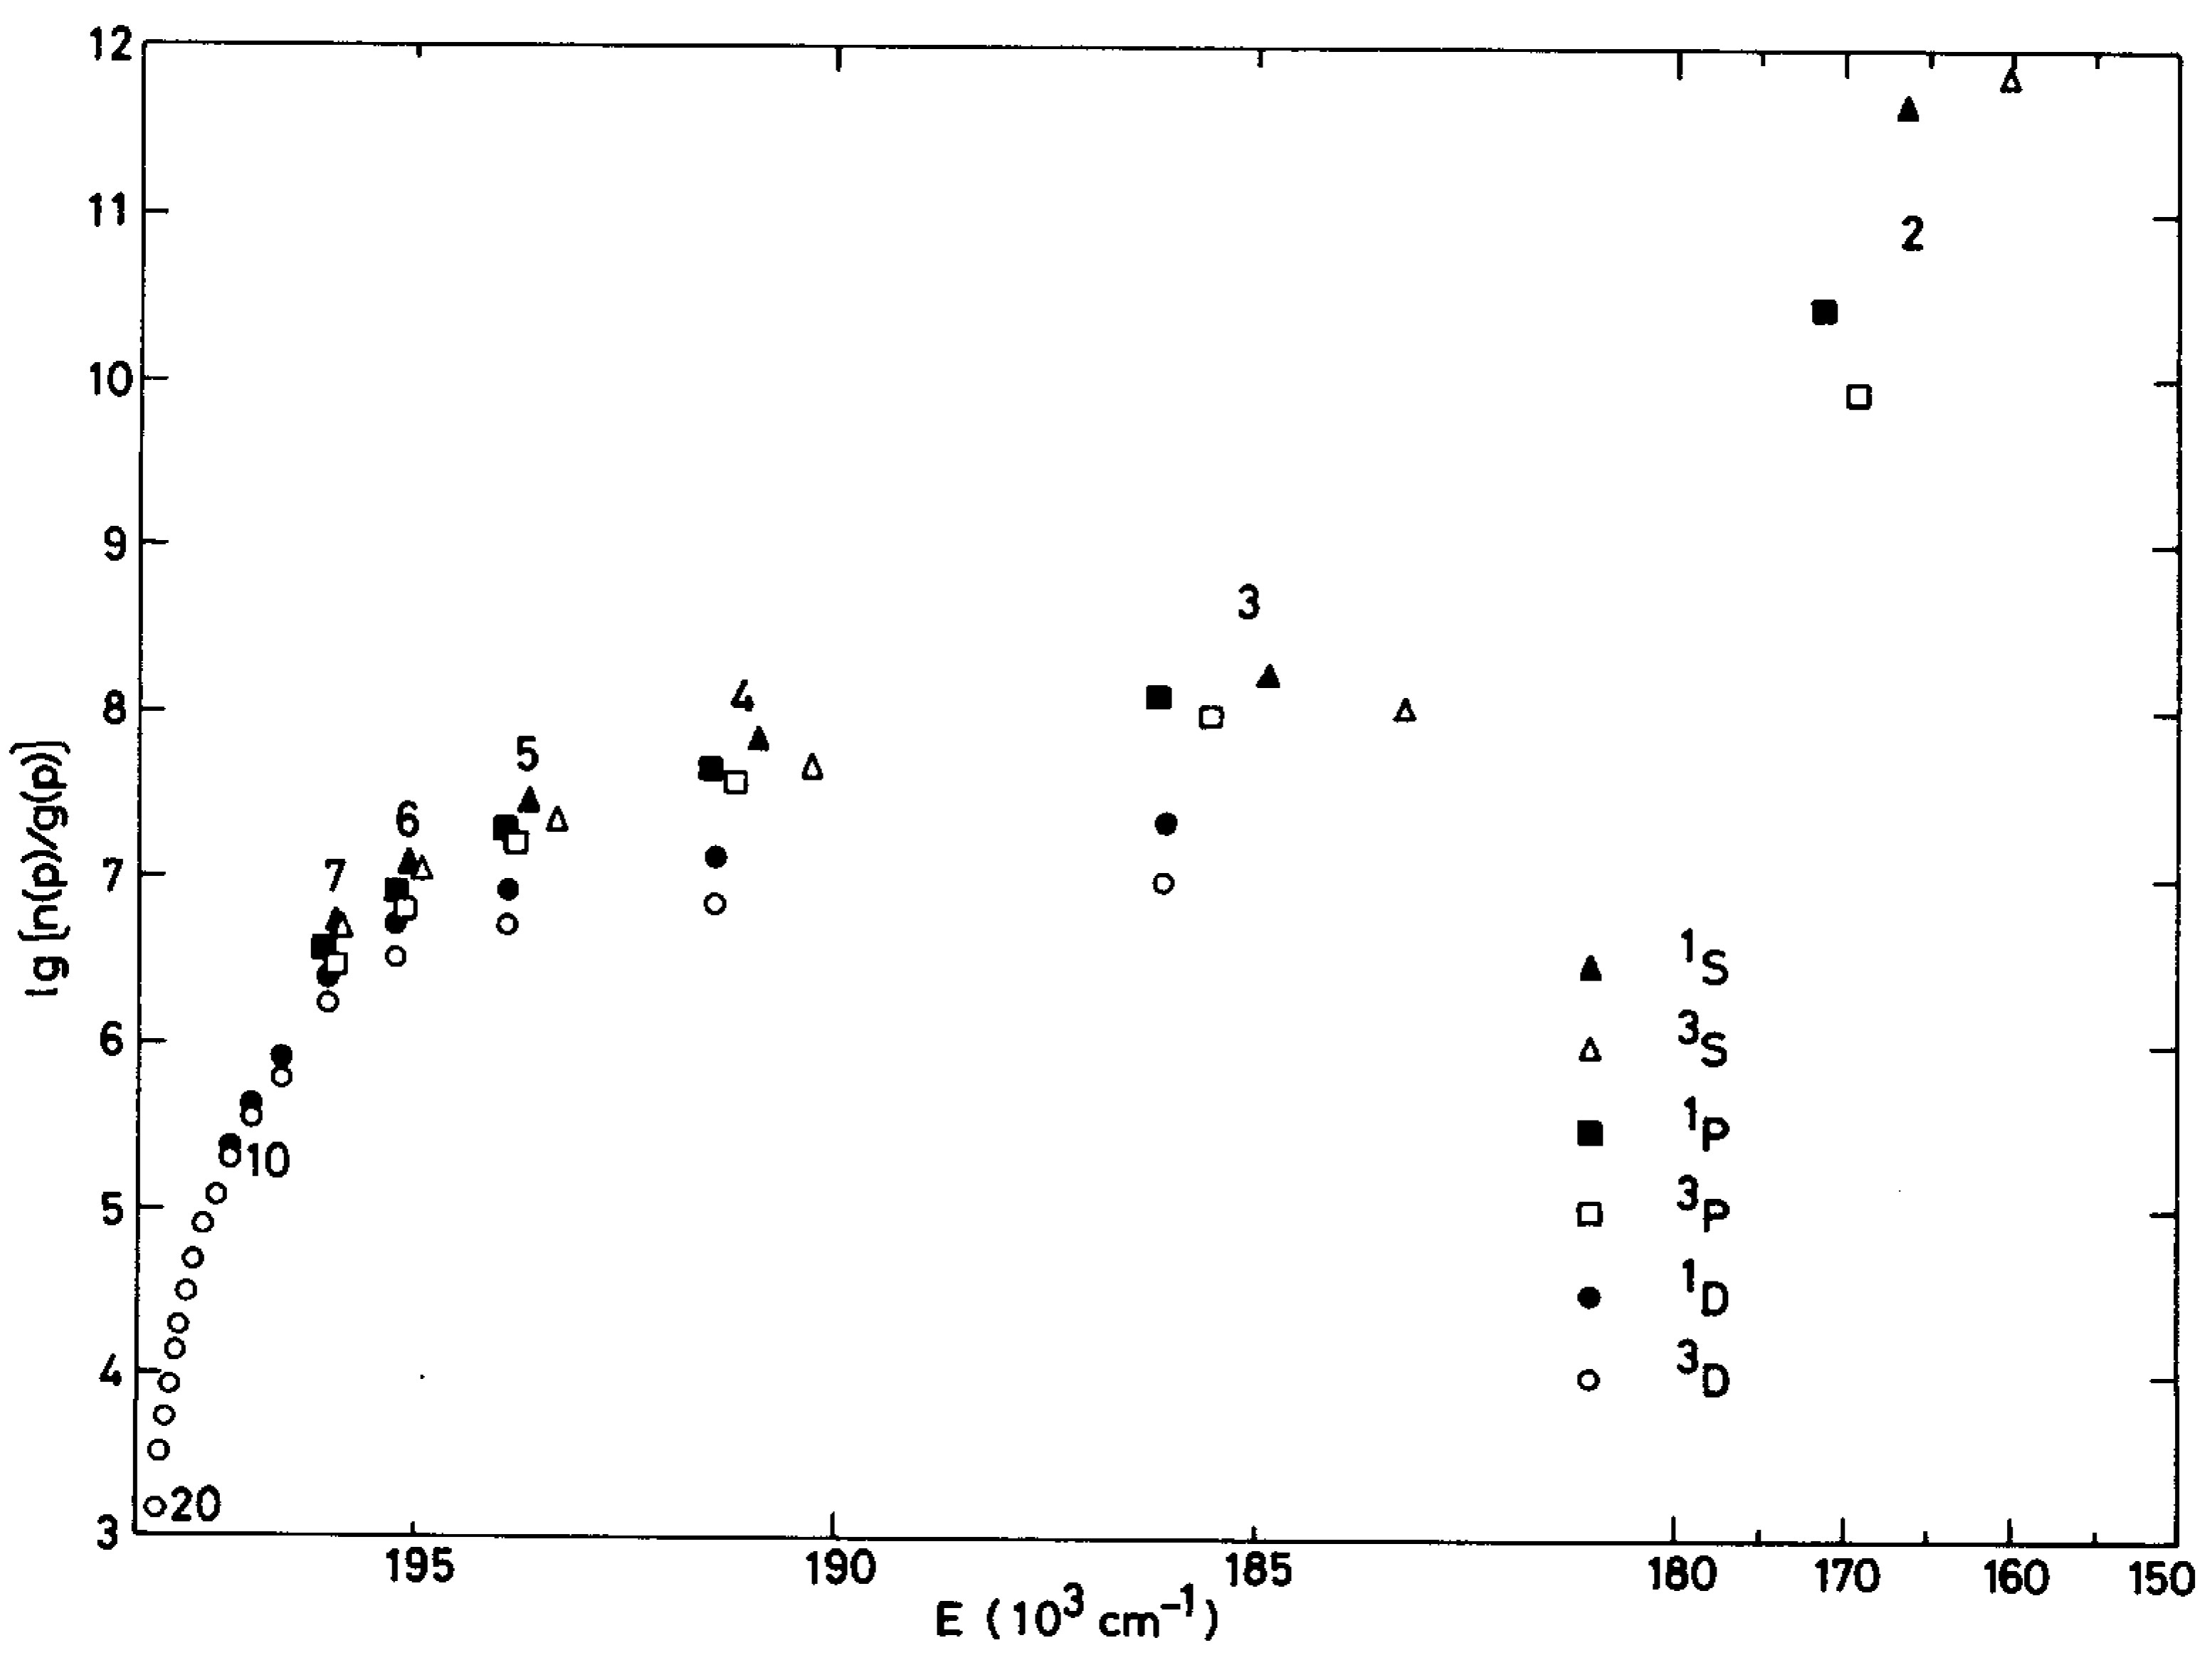
\includegraphics[width=0.7\textwidth]{fujimoto-level-distribution.jpg}
  \caption{T. Fujimoto 对氦原子能级数密度的计算结果。对应放电管(直径 $R=0.8\,{\rm cm}$)实验参数为气压 $53.3\,{\rm Pa}$、放电电流 $100\,{\rm mA}$。放电管中心的基态氦原子数密度为 $1.2\times10^{16}\,{\rm cm}^{-3}$、 电子密度为 $6.3\times10^{10}\,{\rm cm}^{-3}$、 电子温度为 $4.9\,{\rm eV}$。 图片来自\onlinecite{Fujimoto1979-HeCR}。}
  \label{fig:chap03:fujimoto-level-distribution}
\end{figure}

图 \ref{fig:chap03:fujimoto-level-distribution} 显示的是 T. Fujimoto 的碰撞辐射模型\cite{Fujimoto1979-HeCR} 对一个放电管中氦原子能级数密度分布的计算结果。根据 H. R. Griem 提出的原则\cite{Griem1964-book},给出了一个临界能级主量子数:
\begin{equation}\label{eq:chap03:criticalLevel}
    n_c=\left(\frac{8\cdot10^{17}}{N_{\rm e}}\right)^{2/17}
        \left(\frac{kT_{\rm e}}{\chi_H}\right)^{1/17} ,
\end{equation}
其中,$\chi_H$ 为氢的基态电离能,$k$ 为玻尔兹曼常数。主量子数处于 $n_c$ 以下的能级粒子数密度与能级的能量之间无明显的函数关系(除基态与亚稳态外 $N_p/g_p\propto n^{-0.5}$,其中,$N_p$ 与$g_p$ 分别为 $p$ 激发态的数密度和统计权重因子,$n$ 为 $p$ 激发态能级的主量子数),其能级粒子数由激发态粒子之间电子碰撞跃迁与自发辐射过程共同决定,称为日冕区~(corona phase)能级。主量子数处于 $n_c$ 以上能级的粒子数密度随能级的升高而快速下降($N_p/g_p\propto n^{-6}$),其粒子之间的电子碰撞跃迁过程大于自发辐射过程,称为准饱和区(quasi-saturation phase)能级。对于SUNIST 等离子体,在高密度低温等离子体条件下 $n_c=4$;在低密度高温等离子体条件下 $n_c=6$。基于此结论,本文的 CR 模型包含主量子数 $n\le 7$ 的所有激发态能级(第 \ref{sec:chap03:maxn-in-crm} 节将给出更多的讨论)以及氦的两个离子 ${\rm He}^+$ 与${\rm He}^{2+}$,将轨道角动量 $l\ge 3$ 的能级合并成为一个能级,记为 ${\rm F}^+$ 能级。
图 \ref{fig:chap03:he-level-diagram} 所示为本文模型的氦原子能级图。

\begin{figure}
  \centering
  \begin{overpic}[width=0.7\textwidth]{He-diagrames-plus-wlxb-en.pdf}
    \put(20,1){\mbox{\colorbox{white}{\quad 自旋单重态\quad}}}
    \put(60,1){\mbox{\colorbox{white}{\quad 自旋三重态\quad}}}
    \put(-1,32){\rotatebox{90}{\mbox{\colorbox{white}{\quad 能量 (${\rm eV}$)}}}}
    \put(53.7,86.8){$^+$}
    \put(88.9,86.8){$^+$}
  \end{overpic}
  %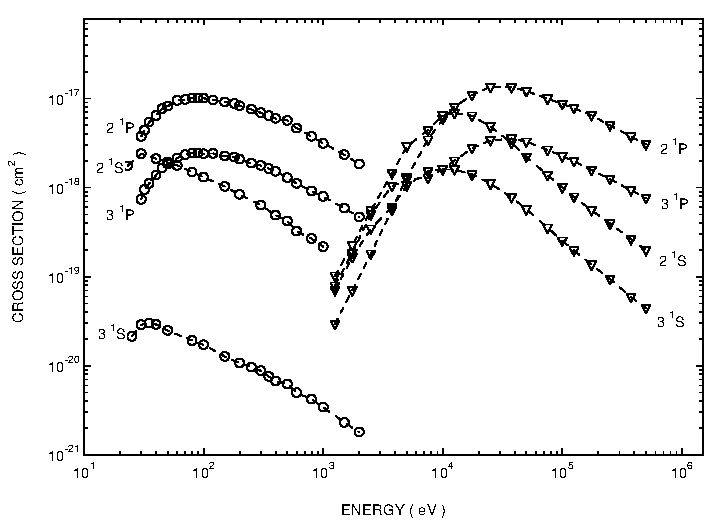
\includegraphics[width=0.7\textwidth]{he-exc-xsec-compare.pdf}
  \caption{本文碰撞辐射模型使用的氦原子能级图。图片来自\onlinecite{xie:wlxb},能级数据来自\onlinecite{NISTdatabase}。}
  \label{fig:chap03:he-level-diagram}
\end{figure}


%\subsection{忽略氢及其他杂质粒子的影响}
%\subsection{SUNIST 等离子体原子反应过程选择及等离子体的光学厚度}

%真空室内的水与氢气是较难去除的。

%\subsection{SUNIST 等离子体原子激发和电离过程的选择}
\subsection{氦原子激发和电离过程的选择}

影响氦原子数密度的首先是碰撞电离过程,可以将氦原子内的电子剥离的反应过程如下\cite{Anderson1999:Thesis}:
\begin{enumerate}
  \item 电子碰撞电离与双电离\\
        ${\rm e}+{\rm He}\to {\rm e}+{\rm He}^+ + {\rm e}$\\
        ${\rm e}+{\rm He}\to {\rm e}+{\rm He}^{2+} + {\rm e} + {\rm e}$
  \item 离子碰撞电离与双电离\\
        ${\rm X}^{+z_0} + {\rm He} \to {\rm X}^{+z_0} + {\rm He}^+ + {\rm e}$\\
        ${\rm X}^{+z_0} + {\rm He} \to {\rm X}^{+z_0} + {\rm He}^{2+} + {\rm e} + {\rm e}$
  \item 单电子与双电子电荷交换\\
        ${\rm X}^{+z_0} + {\rm He} \to {\rm X}^{+z_0-1} + {\rm He}^+ $\\
        ${\rm X}^{+z_0} + {\rm He} \to {\rm X}^{+z_0-2} + {\rm He}^{2+}$
  \item 电子交换双电离(transfer double ionization)\\
        ${\rm X}^{+z_0} + {\rm He} \to {\rm X}^{+z_0-1} + {\rm He}^{2+} + {\rm e}$
\end{enumerate}
其中,${\rm X}$ 表示某杂质原子或离子。

影响氦原子激发态数密度的是碰撞激发、退激发以及自发辐射跃迁过程,其主要反应如下\cite{Anderson1999:Thesis}:
\begin{enumerate}
  \item[5.] 电子与离子碰撞激发与退激发\\
        ${\rm e}+{\rm He}(n\,^{\rm 2S+1}{L}) \leftrightarrow {\rm e}+{\rm He}(n\,^{\rm 2S+1}{L})$\\
        ${\rm X}^{+z_0} + {\rm He}(n\,^{1}L) \leftrightarrow {\rm X}^{+z_0} + {\rm He}(n\,^{1}L)$
  \item[6.] 自发辐射跃迁\\
        ${\rm He}(n\,^{\rm 2S+1}L) \to  {\rm He}(n\,^{\rm 2S+1}L) + h\nu$
\end{enumerate}
其中,电子碰撞可以产生自旋变化跃迁,而离子碰撞只能在相同的自旋能级粒子之间发生跃迁。

以上每个反应过程,对于特定的 $p$ 能级粒子,其粒子数密度 $N_p$ 变化速率为:
\begin{equation}
  \frac{{\rm d}\,N_p}{{\rm d}\,t}=-n_{\rm e,X}\cdot N_p\cdot <v_{\rm e,X}\cdot\sigma_{pq}>
  \label{eq:chap03:p-rate-eq}
\end{equation}
其中,$n_{\rm e,X}$ 为电子或重粒子的数密度,$v_{\rm e,X}$ 为电子或重粒子的碰撞速度,$\sigma_{pq}$ 为 $p\to q$ 反应过程的碰撞截面。可以看出,在碰撞辐射模型中,影响激发态能级粒子数密度的过程主要受 $n_{\rm e,X}$、$N_p$、$v_{\rm e,X}$ 和 $\sigma_{pq}$ 四个因素乘积的影响。下面我们将对这些因素做详细分析,分析过程中将氦原子的基态(${\rm gs}$)、亚稳态(${\rm meta}$)和普通激发态 $p$ 进行分别讨论。

\begin{figure}
  \centering
  \begin{overpic}[width=\textwidth]{rel-levelabun-thesis.pdf}
  \end{overpic}
  %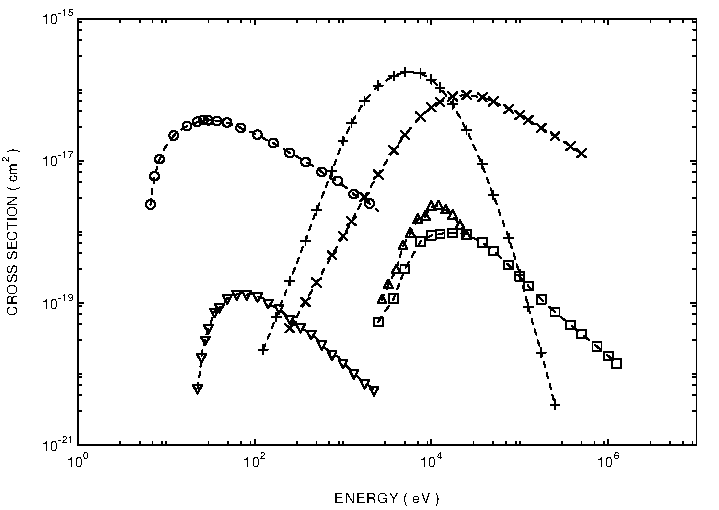
\includegraphics[width=0.7\textwidth]{he-ionization-xsec-comapre.pdf}
  \caption{氦等离子体中 $n\le3$ 各能级和氦离子(${\rm He}^{+}$ 和 ${\rm He}^{2+}$)相对含量随电子温度和电子密度的变化趋势。(a):$T_{\rm e}=20\,{\rm eV}$ 时随电子密度的变化;(b):$N_{\rm e}=1.0\times10^{12}\,{\rm cm}^{-3}$ 时随电子温度的变化。}
  \label{fig:chap03:rel-levelabun-compare}
\end{figure}

1)粒子数密度的量级

图 \ref{fig:chap03:rel-levelabun-compare} 所示为碰撞辐射模型对氦等离子体中 $n\le3$ 各能级粒子和氦离子(${\rm He}^{+}$ 和 ${\rm He}^{2+}$)相对含量随 $T_{\rm e}$ 和 $N_{\rm e}$ 的变化趋势计算结果。可以看出在 SUNIST 等离子体参数范围内,当 $T_{\rm e}=20\,{\rm eV}$ 时,由于电子碰撞激发,普通激发态粒子数密度随 $N_{\rm e}$ 增大而增加,基态和亚稳态由于电子碰撞激发过程的影响,其粒子数密度相对略有下降。在特定的 $N_{\rm e}$ 条件下($1.0\times10^{12}\,{\rm cm}^{-3}$),随着 $T_{\rm e}$ 的上升,各氦原子能级数密度快速下降。我们将以图 \ref{fig:chap03:rel-levelabun-compare}(a) 所示做氦原子和氦离子的数密度量级估计,SUNIST 氦放电等离子体中,可以认为 $N_{\rm e}$ 与 ${\rm He}^{2+}$ 具有相同量级的数密度。

对于 SUNIST 真空室,连续放电后,质谱测量结果显示等效氢原子数占本底原子数约为 $40\%$,为氦等离子体放电时的主要杂质。本底气压在小于 $1\times10^{-4}\,{\rm Pa}$ 范围内,放电时的气压约为 $4.5\times10^{-3}\,{\rm Pa}$,可见,正常放电时 H 的数密度比 $N_{{\rm He}^{2+}}$ 要小两个数量级,同时,由于其他如 C、N、O 等杂质含量不会高于氢\cite{Isler1984:NF:Impurities},我们这里将这些杂质粒子的数密度量级设为与 H 相同。

表 \ref{table:chap03:N-gusuan} 所示为 SUNIST 氦放电等离子体各粒子数密度量级的估算结果,在量级估算时,以基态能级粒子数密度 $N_{\rm gs}$ 为基准。

\begin{table}%[H]
\caption{氦等离子体各粒子数密度的量级}
\label{table:chap03:N-gusuan}
\begin{center}
\begin{tabular}{lcc}\toprule[1.5pt]
粒子数密度 & & 量级 \\
\midrule[1pt]
\hspace{1.5em}$N_{\rm gs}$ & & \hspace{0.5em}$0$ \\
\hspace{1.5em}$N_{\rm meta}$ & & \hspace{0.5em}$-1^{*}$ \\
\hspace{1.5em}$N_p$ & & $-4$ \\
\hspace{1.5em}$N_{{\rm He}^{2+}}$ & & $+6$ \\
\hspace{1.5em}$N_{\rm X}$ & & $+4$ \\
\hspace{1.5em}$N_{\rm e}$ & & $+6$\\
\bottomrule[1.5pt]
\end{tabular}\\[0.5em]
{\small$*$:$-1$ 表示该粒子数密度的量级为基准数密度的 $10^{-1}$。}
\end{center}
\end{table}

2)碰撞速度的量级

对于 SUNIST 等离子体,电子与离子的热平衡弛豫时间常数为 $\tau_{\rm i-e}\sim2\,{\rm ms}$ (第 \ref{sec:chap03:quasi-stationary} 节),与 SUNIST 放电平顶段持续时间相同,可以认为离子温度是远小于电子温度的,则电子与重粒子的碰撞速度应有三个量级的差别。重粒子主要为 H、He、C、N 和 O 等轻元素,不妨认为他们具有相同量级的碰撞速度。以电子碰撞速度 $v_{\rm e}$ 为基准,表 \ref{table:chap03:v-gusuan} 所示为碰撞速度的量级结果。

\begin{table}%[H]
\caption{各粒子碰撞速度的量级}
\label{table:chap03:v-gusuan}
\begin{center}
\begin{tabular}{lcc}\toprule[1.5pt]
碰撞速度 & & 量级 \\
\midrule[1pt]
\hspace{1.5em}$v_{\rm e}$ & & \hspace{0.5em}$0$ \\
\hspace{1.5em}$v_{\rm He}$ & & $-3$ \\
\hspace{1.5em}$v_{\rm X}$ & & $-3$ \\
\bottomrule[1.5pt]
\end{tabular}
\end{center}
\end{table}

3)碰撞截面的量级

\begin{figure}
  \centering
  \begin{overpic}[width=0.7\textwidth]{he-ionization-xsec-comapre.pdf}
    \put(45,1){\mbox{\colorbox{white}{能量 (${\rm eV}$)}}}
    \put(-3,25){\rotatebox{90}{\mbox{\colorbox{white}{碰撞截面 (${\rm cm}^2$)}}}}
  \end{overpic}
  %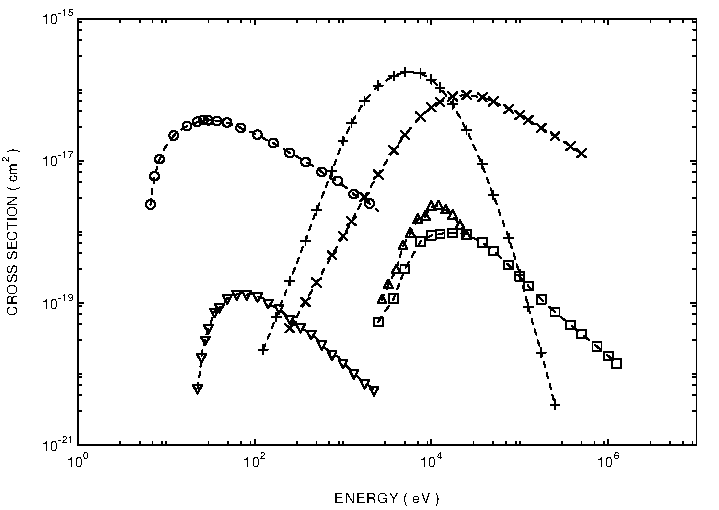
\includegraphics[width=0.7\textwidth]{he-ionization-xsec-comapre.pdf}
  \caption{氦原子基态($1^1{\rm S}$)的电子与氢离子(质子)碰撞电离反应截面数据。$\circ$:电子碰撞电离;$\triangledown$:电子碰撞双电离;$+$:单电子电荷交换;$\times$:质子碰撞电离;$\triangle$:电子交换双电离;$\Box$:质子碰撞双电子电离。图片来自
  \onlinecite{Anderson1999:Thesis}。}
  \label{fig:chap03:he-ion-xsec-compare}
\end{figure}

图 \ref{fig:chap03:he-ion-xsec-compare} 所示为氦原子的电子与质子碰撞电离过程截面数据。可以看出,在几十至几百电子伏的温度范围,电子碰撞电离过程的截面远大于其他反应过程。电子碰撞双电离过程的截面虽然低两个数量级,但也比质子碰撞电离过程截面要大。只有当温度达到 $\sim750\,{\rm eV}$ 及以上时,单电子电荷交换过程才变得重要,并且质子碰撞电离过程与其相当,直到温度达 $20\,{\rm keV}$ 以上,质子碰撞电离过程的截面超过电荷交换过程。

\begin{figure}
  \centering
  \begin{overpic}[width=0.7\textwidth]{he-exc-xsec-compare.pdf}
    \put(45,1){\mbox{\colorbox{white}{能量 (${\rm eV}$)}}}
    \put(-2,25){\rotatebox{90}{\mbox{\colorbox{white}{碰撞截面 (${\rm cm}^2$)}}}}
  \end{overpic}
  %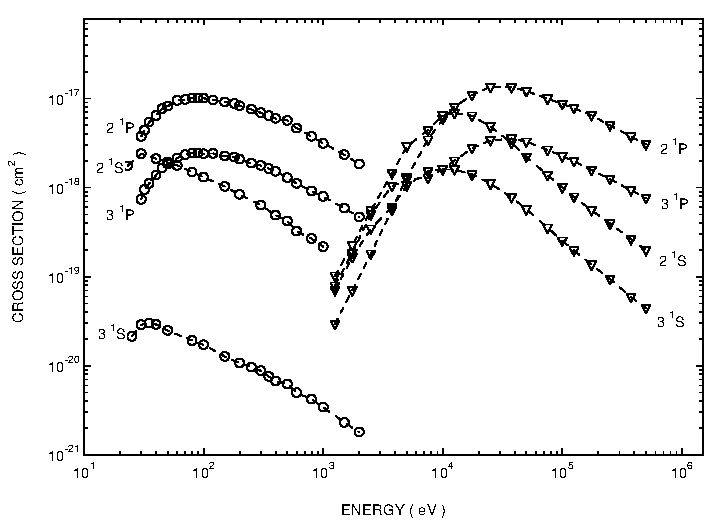
\includegraphics[width=0.7\textwidth]{he-exc-xsec-compare.pdf}
  \caption{氦原子基态($1^1{\rm S}$)的电子与氢离子(质子)碰撞激发截面。$\circ$:电子碰撞激发;$\triangledown$:质子碰撞激发。图片来自\onlinecite{Anderson1999:Thesis}。}
  \label{fig:chap03:he-exc-xsec-compare}
\end{figure}

图 \ref{fig:chap03:he-exc-xsec-compare} 显示的是基态氦原子的电子与质子碰撞激发反应截面。可以看出,只有当温度高于 $1\,{\rm keV}$ 时,质子碰撞激发过程才显得重要。

由此,以电子碰撞激发截面为基准,各激发和电离过程的截面量级在表 \ref{table:chap03:sigma-gusuan} 中列出。

\begin{table}%[H]
\caption{氦原子电子碰撞(${\rm e-}$)和重粒子碰撞(${\rm X-}$)激发、电离过程截面的量级}
\label{table:chap03:sigma-gusuan}
\begin{center}
\begin{tabular}{lcc}\toprule[1.5pt]
碰撞截面$^*$ & & 量级 \\
\midrule[1pt]
\hspace{0.5em}$\sigma_{\rm e-exc}$ & & \hspace{0.5em}$0$ \\
\hspace{0.5em}$\sigma_{\rm X-exc}$ & & $-3$ \\%[1em]
\hspace{0.5em}$\sigma_{\rm e-ion}$ & & $+1$ \\
\hspace{0.5em}$\sigma_{\rm e-dbion}$ & & $-2$ \\
\hspace{0.5em}$\sigma_{\rm X-ion}$ & & $-3$ \\
\hspace{0.5em}$\sigma_{\rm X-dbion}$ & & $-3$ \\
\bottomrule[1.5pt]
\end{tabular}\\[0.5em]
{\small $*$:其中,${\rm exc}$ 表示激发过程,${\rm ion}$ 表示电离过程,${\rm dbion}$ 表示双电子离过程}
\end{center}
\end{table}

4)电子碰撞与重粒子碰撞激发过程的选择

根据表 \ref{table:chap03:N-gusuan} -- 表 \ref{table:chap03:sigma-gusuan},将电子碰撞和重粒子碰撞的氦原子激发过程及其数密度反应速率量级估算结果在表 \ref{table:chap03:exc-process-gusuan} 中列出。可见,氦原子基态的电子碰撞激发过程占主要部分,而普通激发态能级粒子的电子碰撞激发要低四个量级,重粒子碰撞的激发反应速率则更低。所以在碰撞辐射模型中将重粒子碰撞激发过程忽略是合理的。

\begin{table}%[H]
\caption{氦原子电子碰撞(${\rm e-}$)和重粒子碰撞(${\rm X-}$)激发过程的量级估算}
\label{table:chap03:exc-process-gusuan}
\begin{center}
%{\small 其中,${\rm exc}$ 表示激发过程,${\rm ion}$ 表示电离过程,${\rm dbion}$ 表示双电子离过程}\\
\begin{tabular}{lrrrrc}\toprule[1.5pt]
反应过程 & $n_{\rm e,X}$ & $N_{p}$ & $v_{e,X}$ & $\sigma_{pq}$ & 反应过程量级\\
\midrule[1pt]
${\rm e-}$基态       & $+6$ & $0$  & $0$  & $0$  & $+6$ \\
${\rm e-}$亚稳态     & $+6$ & $-1$ & $0$  & $0$  & $+5$ \\
${\rm e-}$普通激发态 & $+6$ & $-4$ & $0$  & $0$  & $+2$ \\
${\rm X-}$基态       & $+4$ & $0$  & $-3$ & $-3$ & $-2$ \\
${\rm X-}$亚稳态     & $+4$ & $-1$ & $-3$ & $-3$ & $-3$ \\
${\rm X-}$普通激发态 & $+4$ & $-4$ & $-3$ & $-3$ & $-6$ \\
\bottomrule[1.5pt]
\end{tabular}
\end{center}
\end{table}

5)电子碰撞与重粒子碰撞电离过程的选择

将电子碰撞和重粒子碰撞的氦原子电离过程及其数密度速率量级估算结果在表 \ref{table:chap03:ion-process-gusuan} 中列出。可见,对于氦的电离过程,在碰撞辐射模型中,将重粒子碰撞电离、双电离以及除基态外的电子碰撞双电离过程忽略是合理的。

\begin{table}%[H]
\caption{氦原子电子碰撞(${\rm e-}$)和重粒子碰撞(${\rm X-}$)电离过程的量级估算}
\label{table:chap03:ion-process-gusuan}
\begin{center}
%{\small 其中,${\rm exc}$ 表示激发过程,${\rm ion}$ 表示电离过程,${\rm dbion}$ 表示双电子离过程}\\
\begin{tabular}{lrrrrc}\toprule[1.5pt]
反应过程 & $n_{\rm e,X}$ & $N_{p}$ & $v_{e,X}$ & $\sigma_{pq}$ & 反应过程量级\\
\midrule[1pt]
${\rm e-}$基态       & $+6$ & $0$  & $0$  & $+1$ & $+7$ \\
${\rm e-}$亚稳态     & $+6$ & $-1$ & $0$  & $+1$ & $+6$ \\
${\rm e-}$普通激发态 & $+6$ & $-4$ & $0$  & $+1$ & $+3$ \\
${\rm X-}$基态       & $+4$ & $0$  & $-3$ & $-3$ & $-2$ \\
${\rm X-}$亚稳态     & $+4$ & $-1$ & $-3$ & $-3$ & $-3$ \\
${\rm X-}$普通激发态 & $+4$ & $-4$ & $-3$ & $-3$ & $-6$ \\
${\rm e-}$基态(双电离)       & $+6$ & $0$  & $0$  & $-2$  & $+4$ \\
${\rm e-}$亚稳态(双电离)     & $+6$ & $-1$ & $0$  & $-2$  & $+3$ \\
${\rm e-}$普通激发态(双电离) & $+6$ & $-4$ & $0$  & $-2$  & \hspace{0.8em}$0$ \\
${\rm X-}$基态(双电离)       & $+4$ & $0$  & $-3$ & $-3$ & $-2$ \\
${\rm X-}$亚稳态(双电离)     & $+4$ & $-1$ & $-3$ & $-3$ & $-3$ \\
${\rm X-}$普通激发态(双电离) & $+4$ & $-4$ & $-3$ & $-3$ & $-6$ \\
\bottomrule[1.5pt]
\end{tabular}
\end{center}
\end{table}

\subsection{氦放电等离子体光学厚度的计算}

根据式 (\ref{eq:chap02:mod}),计算了在不同的温度和密度组合下平均光学厚度 $\tau_0$ 的数值,如表 \ref{table:chap03:helines-mod} 所示。因为 SUNIST 等离子体中较低的 $n_i$ 与较高的 $v_{\rm th}$,SUNIST 等离子体对测量谱线的吸收作用可以忽略,计算结果还显示即使对跃迁低能级为基态或亚稳态的共振线,仍可以忽略等离子体的吸收影响。

\begin{table}%[H]
\caption{本文测量氦原子谱线的平均光学厚度}
\label{table:chap03:helines-mod}
\begin{center}
\begin{tabular}{ccccccc}
\toprule[1.5pt]
\multirow{3}*{跃迁} & \multirow{3}*{$\lambda_{ji,0}$ (${\rm nm}$)} &
\multicolumn{2}{c}{$\tau_0$ ($10^{-7}$)} & & \multicolumn{2}{c}{$\tau_0$ ($10^{-12}$)} \\
\cmidrule[1pt]{3-4} \cmidrule[1pt]{6-7}
 & & \multicolumn{2}{c}{$T_{\rm e}=30\,{\rm eV}$} & & \multicolumn{2}{c}{$T_{\rm e}=300\,{\rm eV}$}\\
 & & $N_{\rm e}=10^{12}\,{\rm cm}^{-3}$ & $10^{13}\,{\rm cm}^{-3}$ && $N_{\rm e}=10^{12}\,{\rm cm}^{-3}$ & $10^{13}\,{\rm cm}^{-3}$ \\
\midrule[1pt]
$2^1{\rm S}\leftarrow3^1{\rm P}$ & 501.6 & 0.005 & 0.005 && 0.032 & 0.032\\
$2^1{\rm S}\leftarrow4^1{\rm P}$ & 396.5 & 0.001 & 0.001 && 0.008 & 0.008\\
$2^1{\rm P}\leftarrow4^1{\rm S}$ & 504.8 & 0.000 & 0.000 && 0.000 & 0.000\\
$2^1{\rm P}\leftarrow4^1{\rm D}$ & 492.2 & 0.000 & 0.000 && 0.000 & 0.002\\
$2^3{\rm S}\leftarrow3^3{\rm P}$ & 388.9 & 0.442 & 0.116 && 0.242 & 0.083\\
$2^3{\rm P}\leftarrow3^3{\rm D}$ & 587.6 & 0.781 & 1.251 && 0.285 & 0.688\\
$2^3{\rm P}\leftarrow4^3{\rm S}$ & 471.3 & 0.004 & 0.006 && 0.001 & 0.003\\
$2^3{\rm P}\leftarrow4^3{\rm D}$ & 447.1 & 0.120 & 0.192 && 0.044 & 0.105\\
$2^3{\rm P}\leftarrow5^3{\rm S}$ & 412.1 & 0.001 & 0.002 && 0.000 & 0.001\\
\bottomrule[1.5pt]
\end{tabular}
\end{center}
\end{table}

\subsection{氦原子能级数密度反应速率方程的建立}

碰撞辐射模型的核心是对模型中包含的粒子列出其数密度反应速率方程,联立这些方程以求得各粒子的数密度。在氦等离子体中,不同的激发态能级具有不尽相同的主要反应过程,例如 ${\rm He}^{2+}$ 粒子不存在双电子复合过程(dielectric recombination)、电子碰撞双电子电离过程只需计入基态粒子等。本文的碰撞辐射模型针对不同的能级也做了相应的处理。

基态氦原子 $1^1{\rm S}$ 的主要损失过程包括电子碰撞激发与电离;主要产生过程包括激发态电子碰撞退激发和自发辐射跃迁以及 ${\rm He}^+$ 离子的辐射复合(radiation recombination)与偶电子复合(dielectric recombination)过程。其粒子数密度 $N_1$ 的速率方程:
\begin{equation}
    \label{eq:crm:gs}
    \begin{aligned}
        \frac{{\rm d}\,N_1}{{\rm d}\,t}=
        &-\left\{\sum_{q>1}C_{1q}+S_{{\rm He}^+}(1)+S_{{\rm He}^{2+}}(1)\right\}N_{\rm e}N_1\\
        &+\sum_{q>1}\left\{C_{q1}N_{\rm e}+A_{q1}\right\}N_q\\
        &+\left\{\beta_{{\rm He}^+}(1)+\beta_{{\rm He}^+,\rm d}(1)\right\}N_{\rm e}N_{{\rm He}^+}
    \end{aligned}
\end{equation}

对于亚稳态 $2^1{\rm S}$ 和 $2^3{\rm S}$,忽略其与普通激发态的电子碰撞双电子电离与偶电子复合过程,则对于氦原子的激发态和亚稳态 $p$,主要损失过程为电子碰撞激发与退激发、自发辐射跃迁与电子碰撞电离过程;主要产生过程为:电子碰撞激发与退激发,自发辐射跃迁与 ${\rm He}^+$ 离子辐射复合过程。其粒子数 $N_p$ 的速率方程:
\begin{equation}
\label{eq:crm:excstate}
\begin{aligned}
\frac{{\rm d}\,N_p}{{\rm d}\,t}=
&-\left\{\sum_{q\ne p}C_{pq}N_{\rm e}+\sum_{q<p}A_{pq}+S_{{\rm He}^+}(p)N_{\rm e}\right\}N_p\\
&+\left\{\sum_{q\ne p}C_{qp}N_{\rm e}+\sum_{q>p}A_{qp}\right\}N_q\\
&+\beta_{{\rm He}^+}(p)N_{\rm e}N_{{\rm He}^+}
\end{aligned}
\end{equation}

${\rm He}^+$~离子的主要损失过程为电子碰撞电离、辐射复合以及偶电子复合过程;主要产生过程为:原子激发态碰撞电离以及 ${\rm He}^{2+}$ 离子复合过程。其粒子数 $N_{{\rm He}^+}$ 的速率方程为:
\begin{equation}
\label{eq:crm:HeII}
\begin{aligned}
\frac{{\rm d}\,N_{{\rm He}^+}}{{\rm d}\,t}=
&-\left\{\sum_{p}\beta_{{\rm He}^+}(p)+\beta_{{\rm He}^+,{\rm d}}(1)+S_{{\rm He}^{2+}}({\rm He}^+)\right\}N_{\rm e}N_{{\rm He}^+}\\
&+N_{\rm e}\sum_{p}S_{{\rm He}^+}(p)N_p+\beta_{{\rm He}^{2+}}({\rm He}^{+})N_{\rm e}N_{{\rm He}^{2+}}
\end{aligned}
\end{equation}

对于 ${\rm He}^{2+}$,其损失主要通过电子碰撞复合至 ${\rm He}^+$ 离子;主要产生过程为基态原子与 ${\rm He}^+$ 离子的电子碰撞电离。其粒子数 $N_{{\rm He}^{2+}}$ 的速率方程为:
\begin{equation}
\label{eq:crm:HeIII}
\begin{aligned}
\frac{{\rm d}\,N_{{\rm He}^{2+}}}{{\rm d}\,t}=
&-\beta_{{\rm He}^{2+}}({\rm He}^{+})N_{\rm e}n_{{\rm He}^{2+}}\\
&+\left\{S_{{\rm He}^{2+}}(1)N_1+S_{{\rm He}^{2+}}({\rm He}^+)N_{{\rm He}^+}\right\}N_{\rm e}
\end{aligned}
\end{equation}

在速率方程 (\ref{eq:crm:gs}) -- (\ref{eq:crm:HeIII}) 中,$q<p$ 表示 $q$ 能级位于 $p$ 能级之下;$A_{pq}$ 为 $p$ 能级到 $q$ 能级跃迁的爱因斯坦系数;$C_{qp}$ 为电子碰撞跃迁速率系数;$S_{{\rm He}^+}(p)$ 与 $S_{{\rm He}^{2+}}(p)$ 分别为粒子 $p$ 电子碰撞电离至 ${\rm He}^+$ 与 ${\rm He}^{2+}$ 离子的速率系数;$\beta_{{\rm He}^+}(p)$、$\beta_{{\rm He}^{2+}}({\rm He}^+)$ 以及$\beta_{{\rm He}^+,{\rm d}}(1)$ 分别为 ${\rm He}^+$ 离子辐射复合速率系数、${\rm He}^{2+}$ 离子复合至 ${\rm He}^+$ 过程的速率系数以及 ${\rm He}^+$ 离子的偶电子复合至基态速率系数。

\subsection{氦原子反应过程速率系数的计算}

1)电子碰撞激发/退激发过程

对于氦原子的基态、亚稳态以及普通激发态其电子碰撞激发速率系数,本文采用 Y. Ralchenko 等人\cite{Ralchenko2008603,NIFS:DATA:059}对多种数据来源的整理并进行拟合的结果。

为了表示方便,使用振子强度(collision strength) $\Omega(E/\Delta E)$ 来对碰撞截面进行解析表达,其中,$E$ 与 $\Delta E$ 分别为碰撞能量与跃迁能量。振子强度与碰撞截面 $\sigma(E, \Delta D)$ 之间的关系为:
\begin{equation}
    \label{eq:chap03:col-strength-xsec}
    \sigma(E, \Delta E)=\pi a_0^2 \frac{{\rm Ry}}{g_i E}\Omega\left(\frac{E}{\Delta E}\right)
\end{equation}
其中,$\pi a_0^2=0.8797\times10^{-16}\,{\rm cm}^2$,$g_i$ 为起始能级的统计权重因子,里德堡能量 ${\rm Ry}=13.6057\,{\rm eV}$。对于不同的跃迁类别,使用不同的方程对振子强度 $\Omega(x)$ ($x=E/\Delta E$) 做了拟合,将从起始($i$)到结束($f$)能级的跃迁 $n_i^{2S_i+1}L_i\to n_f^{2S_f+1}L_f$ 分为三组:

(a) 偶极跃迁(dipole-allowed)过程($\Delta S=0, \Delta L=\pm 1$)
\begin{equation}
    \Omega(x)=\left(A_1\ln(x)+A_2+\frac{A_3}{x}+\frac{A_4}{x^2}+\frac{A_5}{x^3}\right)\left(\frac{x+1}{x+A_6}\right)
\end{equation}

(b) 偶极禁戒(dipole-forbidden)跃迁过程($\Delta S=0, \Delta L\neq\pm 1$)
\begin{equation}
    \Omega(x)=\left(A_1+\frac{A_2}{x}+\frac{A_3}{x^2}+\frac{A_4}{x^3}\right)\left(\frac{x^2}{x^2+A_5}\right)
\end{equation}

(c) 自旋禁戒(spin-forbidden)跃迁过程($\Delta S\neq0$)
\begin{equation}
    \Omega(x)=\left(A_1+\frac{A_2}{x}+\frac{A_3}{x^2}+\frac{A_4}{x^3}\right)\left(\frac{1}{x^2+A_5}\right)
\end{equation}
其中,$A_k$ 为拟合参数,在文献 \onlinecite{Ralchenko2008603,NIFS:DATA:059} 中以列表的形式给出。这些拟合方程仅适用于起始与结束激发态的主量子数小于等于 $4$ ($n_i, n_f\le4$)的跃迁。

对于 $n_i\leq3, n_f\geq5$ 的跃迁,其碰撞截面使用下面的定标关系:
\begin{equation}
    \sigma\left(n_i^{2S_i+1}L_i-n_f^{2S_f+1}L_f, E\right)=
    \left(\frac{4}{n_f}\right)^3\sigma\left(n_i^{2S_i+1}L_i-4^{2S_f+1}L_f,\frac{E}{\epsilon}\right)
\end{equation}
其中,$\epsilon=\Delta E_{if}/\Delta E_{i4}$ 为跃迁能量之比。当跃迁能级的主量子数差别 $\Delta n=n_f-n_i$ 不大时,定标因子 $(4/n_f)^3$ 需要用比值 $(f_{n_il_i;n_fl_f}/f_{n_il_i;4l_f})$ 进行替代,其中 $f_{n_il_i;n_fl_f}$ 表示跃迁 $n_il_i\to n_fl_f$ 的振子强度。

对于 $n_i\geq4,n_f\geq5$ 的跃迁,将角动量进行简并,跃迁的碰撞截面使用下面的半经验公式:
\begin{equation}
    \sigma\left(n_i-n_f\right)=
    3.52\times10^{-16}\left(\frac{{\rm Ry}}{\Delta E_{n_in_f}}\right)^2f_{n_in_f}F(x)\,({\rm cm}^2)
\end{equation}
其中
\begin{equation}
    F(x)=\frac{1}{x}[1-\exp(-\xi(x+1))\ln(x+0.2)],
\end{equation}
\begin{equation}
    x=\frac{E}{\Delta E_{n_in_f}},\xi=\frac{1}{2}\left(f_{n_in_f}\frac{\rm Ry}{\Delta E_{n_in_f}}\right)^{-0.7}
\end{equation}
并且 $\Delta E_{n_in_f}$ 与 $f_{n_in_f}$ 分别为 $n_i\to n_f$ 跃迁过程的跃迁能量与振子强度,而振子强度 $f_{n_in_f}$ 由文献 \onlinecite{Johnson1972:collisionalstrength} 给出。

对于电子碰撞退激发过程($f\to i$)的速率系数 $C_{fi}$,由精细平衡原理\cite{Lieberman2005-book} 给出\cite{Burgess1992:collisionalstrength}:
\begin{equation}
    C_{fi}=\left(\frac{g_i}{g_j}\right)\exp\left(\frac{\Delta E}{kT}\right)C_{ij}
\end{equation}
其中,$kT$ 为电子温度。

根据式 (\ref{eq:chap03:col-strength-xsec}),碰撞激发的速率系数可以写为\cite{Burgess1992:collisionalstrength}:
\begin{equation}
    C_{ij}=2\pi^{1/2}a_0\hbar m_e^{-1}\left(\frac{\rm Ry}{kT}\right)^{1/2}\exp\left(-\frac{\Delta E}{kT}\right)\frac{\Upsilon_{ij}}{g_i}
\end{equation}
其中,$2\pi^{1/2}a_0\hbar m_e^{-1}=1.1716\times10^{-8}\,{\rm cm}^3{\rm s}^{-1}$,而 $\Upsilon_{ij}$ 为热平均的碰撞振子强度\cite{Seaton07071953}:
\begin{equation}
    \Upsilon_{ij}=\int_0^\infty\Omega_{ij}\exp\left(-\frac{E_f}{kT}\right){\rm d}\left(\frac{E_f}{kT}\right)
\end{equation}
其中, $E_f$ 为碰撞后的电子能量。

在计算麦克斯韦电子温度分布的热平均振子强度值时,本文使用 20 阶的高斯---拉盖尔积分(Gauss-Laguerre quadrature)\cite{GL:url:1,GL:url:2}:
\begin{equation}
    \int_a^{+\infty}|x-a|^\alpha\exp(-b(x-a))f(x)\,{\rm d}x
\end{equation}
进行数值计算。

2)电子碰撞电离过程

对于 $n\leq4$ 的氦原子激发态,其电子碰撞单电离碰撞截面可以由下面的形式进行拟合\cite{Ralchenko2008603,NIFS:DATA:059}:
\begin{equation}
    \sigma_{\rm ion}(n^{2S+1}L)=\frac{10^{-13}}{IE}\left[A_1\ln\frac{E}{I}+\sum_{i=2}^{6}A_i\left(i-\frac{I}{E}\right)^{i-1}\right]\,({\rm cm}^2)
\end{equation}
其中,$I$ 为能级的电离能、$E$ 为碰撞能量、$A_i$ 为拟合系数。基态氦原子的电子碰撞双电离截面也可以由此公式给出。

对于 $n\geq5$ 的激发态,%可以将其简并,电离碰撞截面可以使用以下公式:
%\begin{equation}
%    \sigma_{\rm ion}(n;E)=2.32\times10^{-16}\left(\frac{\rm Ry}{I_n}\right)^2
%    \left(\frac{x-1}{x^2}\right)\ln(1.25x)\,({\rm cm}^2)
%\end{equation}
%其中,$I_n$ 为 $n$ 能级的(平均)电离能,且 $x=E/I_n$。
如果激发态能级的主量子数 $n$ 不太高,对于非简并能级 $n^{2S+1}L$ 的碰撞截面可以使用以下的定标关系:
\begin{equation}
    \sigma_{\rm ion}(n^{2S+1}L;E)=\varepsilon^2\sigma_{\rm ion}(4^{2S+1}L;E/\varepsilon)
\end{equation}
其中,$\varepsilon=I_{4LS}/I_{nLS}$,而 $I_{nLS}$ 为 $n^{2S+1}L$ 能级的电离能。

3)离子复合过程

氦离子(${\rm He}^+$ 和 ${\rm He}^{2+}$)的辐射复合速率系数由以下拟合公式给出
\cite{Verner1996}:
\begin{equation}
    \beta_{\rm r}(T)=a\left[\sqrt{T/T_0}\left(1+\sqrt{T/T_0}\right)^{1-b}\left(1+\sqrt{T/T_1}\right)^{1+b}\right]^{-1}
\end{equation}
其中,$a$、$b$、$T_0$ 与 $T_1$ 为拟合系数,而 $T$ 为电子温度。

氦离子 ${\rm He}^+$ 的偶电子复合速率系数由以下拟合公式给出\cite{Aldrovandi1973,Shull1982,Arnaud1985}:
\begin{equation}
    \beta_{\rm d}(T)=AT^{-3/2}\exp\left(\frac{-T_0}{T}\right)\left[1+B\exp\left(-\frac{T_1}{T}\right)\right]
\end{equation}
其中,$A$、$B$、$T_0$ 与 $T_1$ 为拟合系数。

4)自发辐射跃迁

激发态原子的自发辐射跃迁速率系数(爱因斯坦系数)可以以非常高的精度给出\cite{NISTdatabase}。

综合考虑,氦的电子碰撞速率系数精度总结在表 \ref{tab:chap03:rate-uncertainty} 中。

\begin{table}
\caption{本文使用的电子碰撞速率系数不确定性范围}
\label{tab:chap03:rate-uncertainty}
\begin{center}
\begin{tabular}{L{11em}c}
\toprule[1.5pt]
        \hspace{2em}跃迁类型 & 不确定性\\
\midrule[1pt]
        基态 $\rightarrow$ 自旋单重态 & $\pm10\%$\\ %\addlinespace[.5em]
        基态 $\rightarrow$ 自旋三重态 & $\pm15\%$\\
        亚稳态 $\rightarrow$ 所有激发态 & $\pm20\%$\\
        $n\leq4$ 激发态 $\to$ ${\rm He}^+$ & $\pm15\%$ \\
        基态 $\to$ ${\rm He}^{2+}$ & $\pm11\%$ \\
        氦离子辐射复合 & $\pm10\%$\\
        ${\rm He}^+$ 偶电子复合 & $\pm10\%$\\
        其他过程 & $\pm50\%$\\
\bottomrule[1.5pt]
\end{tabular}
\end{center}
\end{table}

\subsection{对反应速率方程的准稳态近似}
\label{sec:chap03:quasi-stationary}

等离子体中影响激发态数密度的各物理过程弛豫时间常数分为两类\cite{Summers2006},第一类为内在(intrinsic)时间常数,只与原子结构本身有关,主要包括亚稳态辐射弛豫时间 $\tau_{\rm meta-rad}$,普通激发态辐射弛豫时间 $\tau_{\rm ord-rad}$ 与辐射或俄歇自发电离时间 $\tau_{\rm rad-ion}$ 等。他们之间的典型关系:
\begin{equation}
    \tau_{\rm rad-ion}\sim 10^{-13}\,{\rm s}\ll
    \tau_{\rm ord-rad}\sim \frac{10^{-8}}{z^4}\,{\rm s}\ll
    \tau_{\rm meta-rad}\sim \frac{10^1}{z^8}\,{\rm s}
\end{equation}
其中,$z$ 为电荷数。

第二类为外在(extrinsic)时间常数,受到等离子体条件,尤其是 $N_{\rm e}$ 与 $T_{\rm e}$ 的影响,主要包括粒子之间的热平衡弛豫时间(电子--电子 $\tau_{\rm e-e}$、离子--离子 $\tau_{\rm i-i}$、 电子--离子 $\tau_{\rm i-e}$)和电荷变化过程时间常数(如电离与复合过程的时间常数 $\tau_{\rm ion}\sim\tau_{\rm rec}$)等。在 SUNIST 等离子体参数下他们之间的典型关系如下:
\begin{equation}
    \tau_{\rm e-e}\sim 4\,\mu{\rm s}\ll
    \tau_{\rm i-i}\sim 20\,\mu{\rm s}\ll
    \tau_{\rm ion}\sim 1.4-140\,\mu{\rm s}\ll
    \tau_{\rm i-e}\sim 2\,{\rm ms}
\end{equation}

我们将这些时间常数与一个等离子体时间参数 $\tau_{\rm plasma}$ \pozhehao 等离子体在空间尺度上扩散、输运等过程的时间常数\pozhehao 进行对比,对于 SUNIST 欧姆放电等离子体:
\begin{equation}
\label{eq:chap03:time-constant-compare}
    \tau_{\rm ord-rad}\ll
    \tau_{\rm e-e,i-i}\ll
    \tau_{\rm ion}\ll
    \tau_{\rm plasma}
\end{equation}
其中,$\tau_{\rm ion}$ 大于 $\tau_{\rm e-e,i-i}$ 意味着电子与离子分别为麦克斯韦分布;$\tau_{\rm ion}$ 小于 $\tau_{\rm plasma}$(对于 SUNIST 欧姆放电等离子体 $\tau_{\rm plasma}\sim0.3\,{\rm ms}$,详见第 \ref{sec:chap04:sunist-spec-measurements} 节)意味着等离子体在空间尺度上扩散、输运等过程慢于等离子体内原子碰撞辐射反应过程,因此在局域等离子体的碰撞辐射模型计算中可以不考虑等离子体参数随扩散、输运等过程的变化,即,在局部区域内等离子体的原子反应过程可以认为处于准稳态情况。

式 (\ref{eq:crm:gs}) -- (\ref{eq:crm:HeIII}) 描述了氦原子各能级以及氦离子的粒子数密度随时间的变化。准稳态近似条件下可以计算系统达到稳态时的结果。本文稳态情况下的碰撞模型只适合 SUNIST 放电平顶段的等离子体(第 \ref{sec:chap04:sunist-spec-measurements} 节),即可以用来进行托卡马克物理研究的放电阶段。

\subsection{等效电荷数计算结果与 FLYCHK 的对比}
\label{sec:FLYCHK-compare}

\begin{figure}
  \centering
  \begin{overpic}[width=0.5\textwidth]{ZvsTe-spec-Ne-1_0E2_thesis.pdf}
    %\put(48,1){\mbox{\colorbox{white}{$T_{\rm e} (${\rm eV}$)$}}}
  \end{overpic}
  %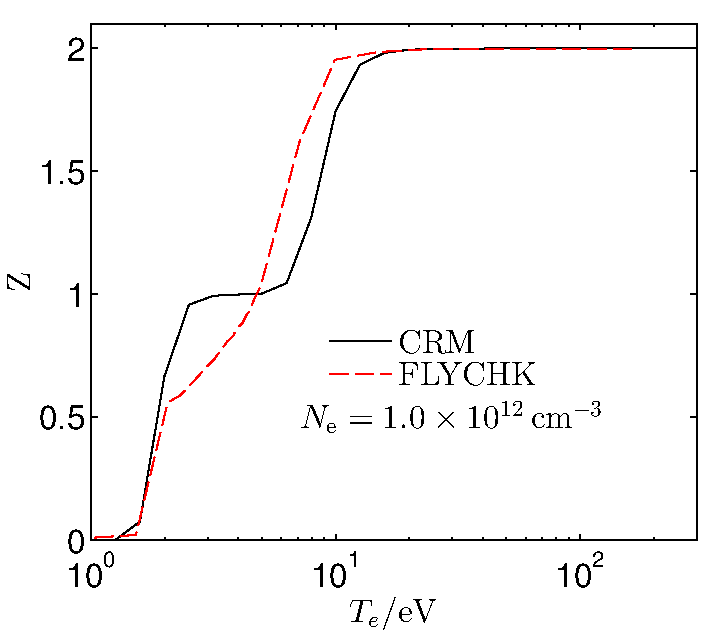
\includegraphics[width=0.5\textwidth]{ZvsTe-spec-Ne-1_0E2.pdf}
  \caption{氦等离子体稳态时平均电荷数与电子温度 $T_{\rm e}$ 的关系。实线为本文碰撞辐射模型计算结果,虚线为 FLYCHK 的计算结果。图片修改自 \onlinecite{xie:wlxb}。}
  \label{fig:chap03:ZvsTe}
\end{figure}

做为对比,图 \ref{fig:chap03:ZvsTe} 给出了在电子密度 $N_{\rm e}=1.0\times10^{12}\,{\rm cm}^{-3}$ 条件下,当达到稳态时, 本文碰撞辐射模型与 FLYCHK\cite{FLYCHK,FLYCHK:url} 代码计算的平均电荷数 $\overline{Z}$ 随 $T_{\rm e}$ 的变化曲线。由图可知,当 $T_{\rm e}>10\,{\rm eV}$ 时,本论文模型与 FLYCHK 的计算结果可以吻合,等离子体中的氦原子已经几乎达到完全电离的状态。两模型的计算结果在 $T_{\rm e}=2\,{\rm eV}-10\,{\rm eV}$ 范围内有最大约 $30\%$ 的误差,这主要是因为两者使用的电子碰撞截面不同造成的。当 $T_{\rm e}$ 在跃迁能量附近时,碰撞反应截面具有比较复杂的行为,无论理论计算还是实验测量都难以获得满意的结果 \cite{Ralchenko2008603},本论文模型计算结果在 $T_{\rm e}=2.5\,{\rm eV}-6\,{\rm eV}$ 的阶梯也可能是由所使用的碰撞截面拟合公式较差的精度造成的。

%\section{SUNIST 氦原子碰撞辐射模型研究}
\section{氦原子碰撞辐射模型的研究}

%\subsection{能级数密度计算结果}


\subsection{各激发态能级的主要产生过程研究}
\label{sec:main-inflow}

通过各能级的主要产生与损失过程可研究 SUNIST 参数下的氦放电等离子体原子的反应特点,如图 $\ref{fig:chap03:main-inflow}$ 所示为超过各能级总产生速率 $10\%$ 的粒子流示意图。因为 SUNIST 主要使用 $n=4$ 能级的原子谱线进行诊断,$n=4$ 各能级的粒子产生流单独画出,而将 $n=3$ 和 $n\ge5$ 的能级分别合并为 $3^1{\rm L}$、$3^3{\rm L}$ 与 $^1hl$、$^3hl$ 能级。

\begin{figure}
    \centering
%    \begin{subfigure}{0.45\columnwidth}
%        \fbox{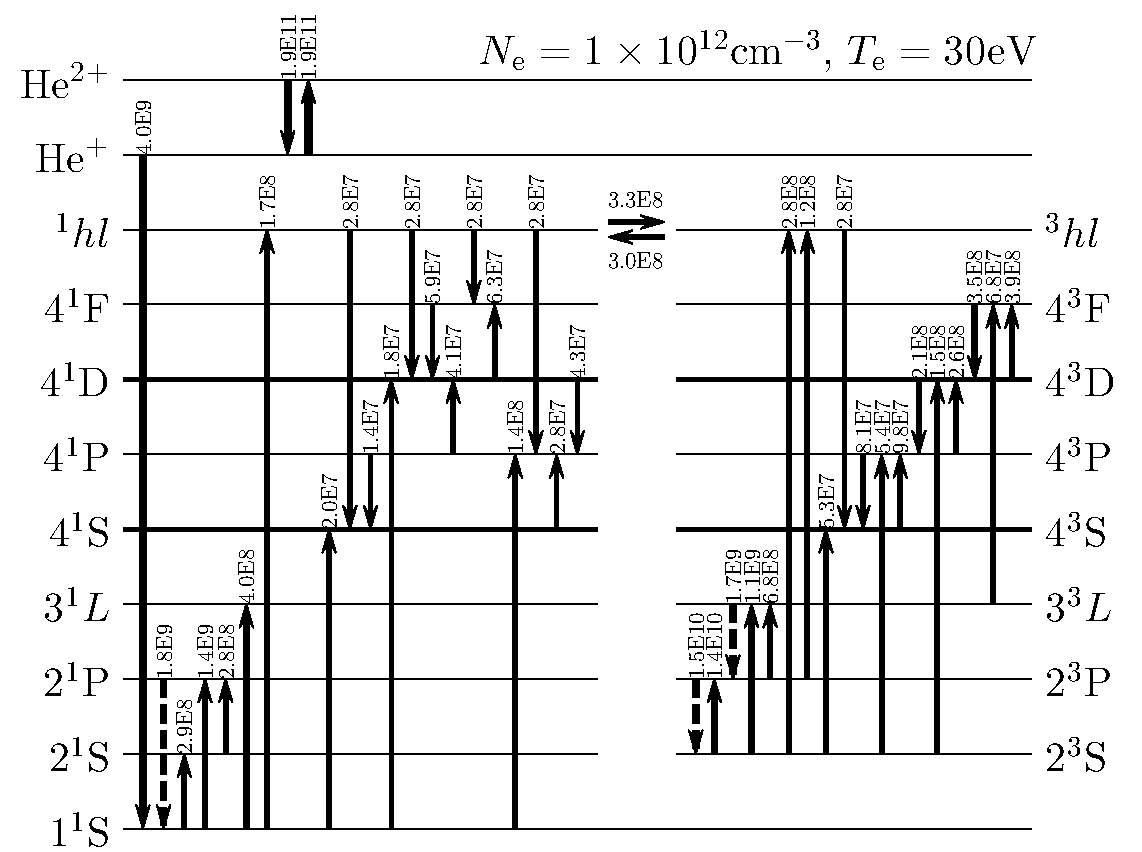
\includegraphics[width=\columnwidth]{Ne1E12_Te30_1e7cm-3s-1.pdf}}
%        \caption{}%
%        \label{fig:chap03:main-inflow:1}
%    \end{subfigure}
%    \hspace{0.05\textwidth}
%    \begin{subfigure}{0.45\columnwidth}
%        \fbox{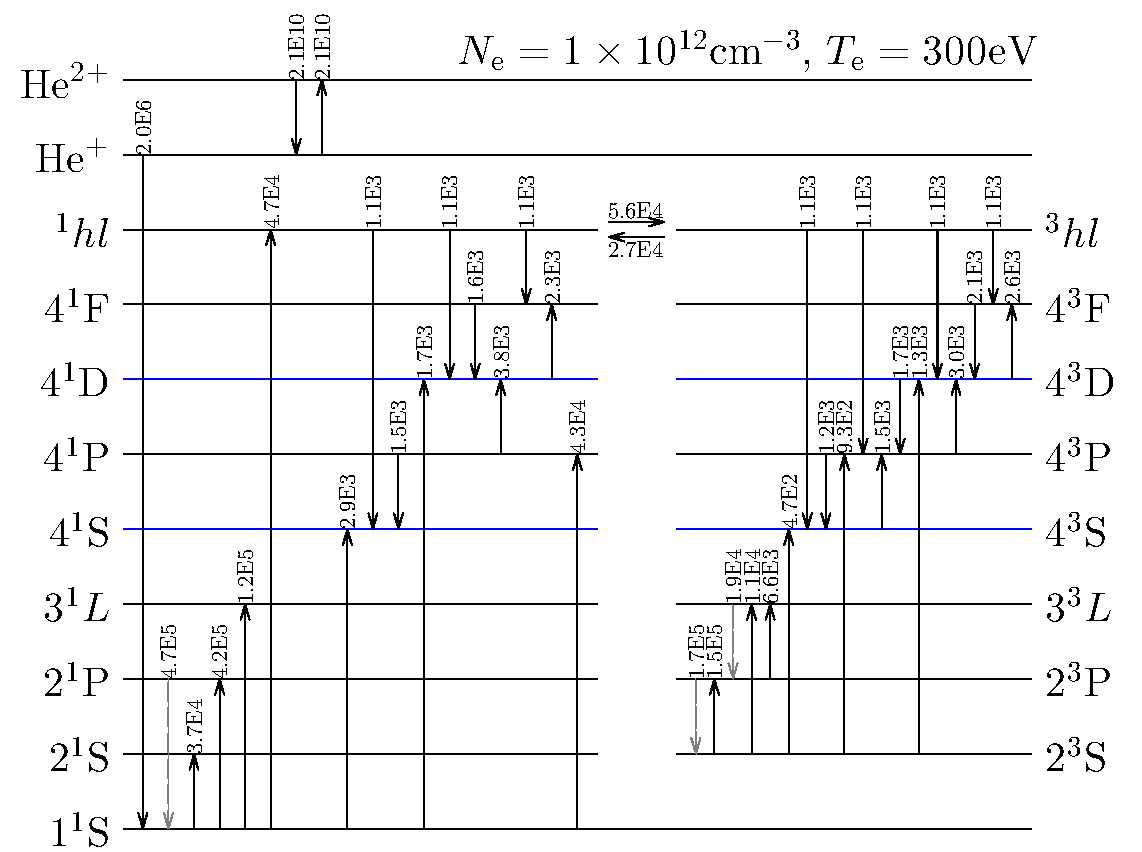
\includegraphics[width=\columnwidth]{Ne1E12_Te300_1e7cm-3s-1.pdf}}
%        \caption{}%
%        \label{fig:chap03:main-inflow:2}
%    \end{subfigure}\\
%    \begin{subfigure}{0.45\columnwidth}
%        \fbox{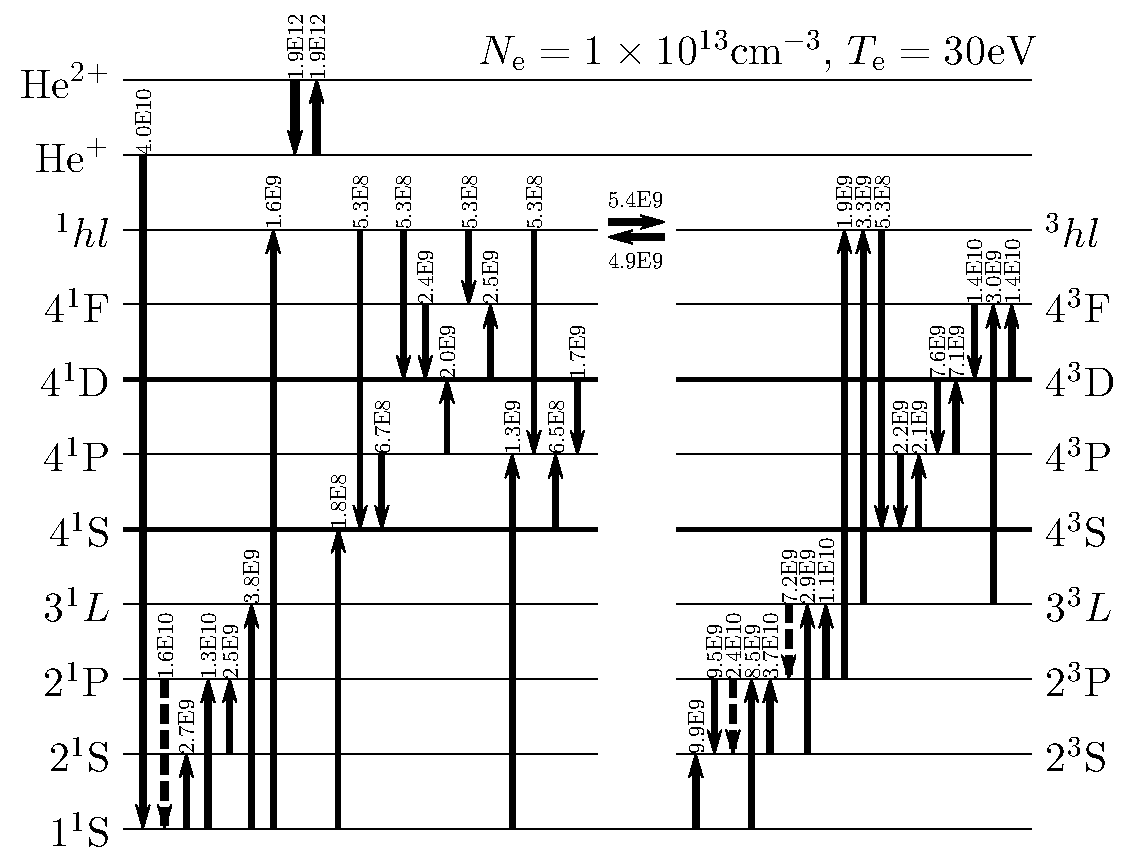
\includegraphics[width=\columnwidth]{Ne1E13_Te30_1e7cm-3s-1.pdf}}
%        \caption{}%
%        \label{fig:chap03:main-inflow:3}
%    \end{subfigure}
%    \hspace{0.05\textwidth}
%    \begin{subfigure}{0.45\columnwidth}
%        \fbox{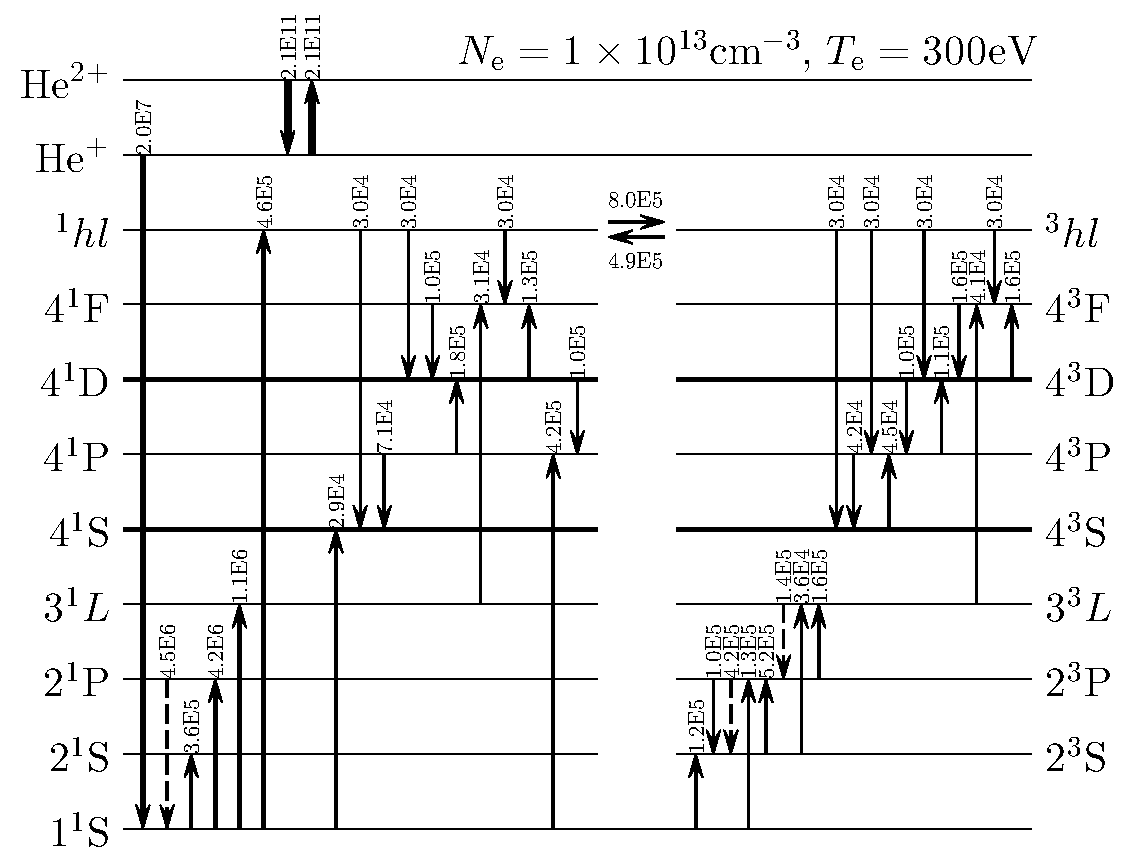
\includegraphics[width=\columnwidth]{Ne1E13_Te300_1e7cm-3s-1.pdf}}
%        \caption{}%
%        \label{fig:chap03:main-inflow:4}
%    \end{subfigure}
    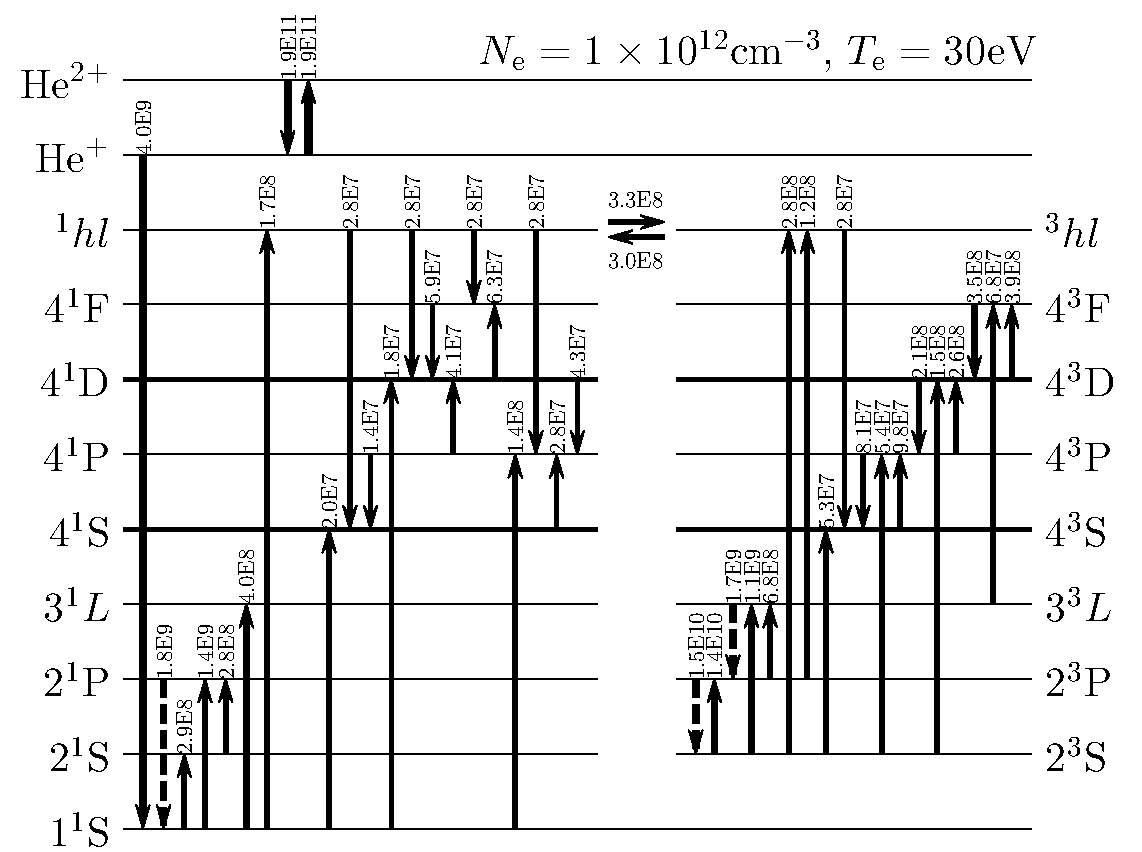
\includegraphics[width=0.8\textwidth]{Ne1E12_Te30_1e7cm-3s-1.pdf}
    \caption{根据碰撞辐射模型结果,
    %不同 $T_{\rm e}$ 和 $N_{\rm e}$ 参数下,
    各能级的主要产生(占比大于该能级总产生速率的 $10\%$)过程。%其中,主量子数 $n\geq 5$ 的能级合并为一个高能级 $hl$。
    其中,虚线箭头为自发辐射跃迁过程,实线箭头为碰撞跃迁过程。}%
    \label{fig:chap03:main-inflow}
\end{figure}

在 $N_{\rm e}=1\times10^{12}\,{\rm cm}^{-3},\,T_{\rm e}=30\,{\rm eV}$ 条件下,$4^1{\rm S}$ 与 $4^1{\rm D}$ 能级的主要产生粒子流来自基态激发、自旋单态高能级 $^1hl$ 退激发以及来自 $n=4$ 的相邻能级的粒子重分配(redistribution),对于$4^3{\rm S}$ 与 $4^3{\rm D}$ 能级,亚稳态 $2^3{\rm S}$ 则取代基态能级,成为主要产生过程的来源之一。另外,对于普通激发态能级,电子碰撞电离与复合过程的产生粒子流不会超过总产生速率流量的10\%。

基态能级粒子的产生主要来自 ${\rm He}^+$ 的复合过程(超过 $80\%$),$2^1{\rm P}$ 能级的共振线辐射也贡献了约 $20\%$ 的粒子产生流,基态的损失则主要由电子碰撞激发至更高能级粒子贡献。亚稳态 $2^3{\rm S}$ 粒子一部分来自基态的自旋变化激发过程,一部分来自其它自旋三重态能级的退激发过程产生。高激发态能级($n\ge5$)粒子则在氦离子与 $n\le4$ 激发态之间起到了桥梁作用。由第 \ref{sec:FLYCHK-compare} 节,氦等离子体的电离率很高,${\rm He}^+$ 与 ${\rm He}^{2+}$ 离子之间的电离与复合过程占了最主要的反应过程部分。

其他 $T_{\rm e}$ 和 $N_{\rm e}$ 条件下的情况与此类似(附录 \ref{appendix:main-inflow}),只是在更高电子密度情况下,基态的电子碰撞激发至 $2^3{\rm S}$ 过程显得更为明显。

\subsection{速率系数不确定性到激发态数密度计算误差传递的研究}
\label{sec:chap04:uncertainty-transport}

碰撞辐射模型中使用的速率系数任何不确定性的存在,都会传递给模型对能级数密度的计算。模型中包含着众多能级粒子与复杂的反应过程,并且相互耦合,现阶段缺乏直接有效的手段对速率系数不确定性的影响进行估计。通常的做法是,对某反应过程的速率系数进行相应扰动,重新计算碰撞辐射模型的速率方程,以观察扰动后的计算结果相对原来的变化\cite{Andrew2000PPCFSensitivity}。

%基于激发态主要产生过程的分析,对于普通激发态(如 $n=4$),其电子碰撞电离与复合过程都不会高于该能级总损失或产生速率的 $10\%$。则在准稳态情况下,对于 $p$ 激发态能级,如下的方程可以成立:
%\begin{equation}
%N_{\rm e}\sum_{i\ne p}C_{ip}N_i=N_{\rm e}N_p\sum_{i\ne p}C_{pi}+N_p\sum_{i<p}A_{pi}
%\label{eq:error:rateequation}
%\end{equation}
%其中 $i$ 可以通过电子碰撞激发或退激发过程可以直接与 $p$ 能级联系的激发态能级粒子。$C_{ip}$、$C_{pi}$ 与 $A_{pi}$ 分别表示电子碰撞产生、损失与自发退激辐射速率系数。而 $i$ 与 $p$ 能级的粒子数密度分别记为$N_i$ 和 $N_p$。由方程 (\ref{eq:error:rateequation}) 可以得出:
%\begin{equation}
%N_p=\frac{N_{\rm e}\sum_{i\ne p}C_{ip}N_i}{N_{\rm e}\sum_{i\ne p}C_{pi}+\sum_{i<p}A_{pi}}
%\label{eq:error:Np}
%\end{equation}
%估计由速率系数不确定性 $s(C_{ip})$ 对 $p$ 能级粒子数引起的最大相对误差\cite{YuChangxuan:book}。 则:
%\begin{eqnarray}
%s_{N_p}=\frac{{\rm d}N_p}{N_p} = s\left(N_{\rm e}\sum_{i\ne p}C_{ip}N_i\right) + s\left(N_{\rm e}\sum_{i\ne p}C_{pi}+\sum_{i<p}A_{pi}\right)% \nonumber \\
%% & = & \frac{}{} + \frac{}{}
%\label{eq:error:EqOrig}
%\end{eqnarray}
%经过推导(附录 \ref{appendix:error-propagate}),可以得出:
%\begin{eqnarray}
%s_{N_p}=E_{jp}\cdot s(C_{jp})=2\frac{f_{jp}}{F_{p,{\rm in}}}s(C_{jp})
%\label{eq:error:Propagation}
%\end{eqnarray}
%其中
%\begin{eqnarray}
%E_{jp}=2\frac{f_{jp}}{F_{p,{\rm in}}}
%\label{eq:error:Propagation}
%\end{eqnarray}
%为 $j\to p$ 反应过程的速率系数不确定性传递函数,其中 $f_{jp}$ 与 $F_{p,{\rm in}}$ 分别表示 $j\to p$ 能级粒子的产生速率与 $p$ 能级的总粒子产生速率。

普通激发态(如 SUNIST 使用的 $n=4$ 能级)具有可以用来进行谱线诊断的谱线辐射,碰撞辐射模型对这些能级的计算精度是我们所主要关注的。因此,在速率系数不确定性传递的推导过程中,我们主要关注这些激发态能级的数密度。为了简化问题,在所有的感兴趣能级产生过程中,考虑同时只有其中某一个过程 $j\to p$ 的速率系数 $C_{jp}$ 具有不确定性\cite{Andrew2000PPCFSensitivity},研究其对感兴趣能级粒子数密度 $N_p$ 引起的相对误差。

由第 \ref{sec:main-inflow} 节对能级主要产生过程的分析我们可以得到,对于普通激发态能级,无论是电子碰撞复合产生过程,还是电离过程的数密度损失速率,都不足以超过其产生或损失总粒子数速率。所以,对于准稳态情况下的等离子体,$p$ 能级离子的总产生速率与总损失速率相等,则:
\begin{equation}
N_{\rm e}\sum_{i\ne p}C_{ip}N_i=N_{\rm e}N_p\sum_{i\ne p}C_{pi}+N_p\sum_{i<p}A_{pi}
\label{eq:appendix:error:rateequation}
\end{equation}
其中 $i$ 表示与 $p$ 能级发生电子碰撞激发、退激发或自发辐射过程的能级;$C_{ip}$、$C_{pi}$ 与 $A_{pi}$ 分别为 $p$ 能级的电子碰撞产生,损失与自发辐射速率系数;而电子密度、$i$ 能级与 $p$ 能级的粒子数密度分别记为 $N_{\rm e}$、$N_i$ 与 $N_p$。

从式 (\ref{eq:appendix:error:rateequation}) 可以解出 $N_p$:
\begin{equation}
N_p=\frac{N_{\rm e}\sum_{i\ne p}C_{ip}N_i}{N_{\rm e}\sum_{i\ne p}C_{pi}+\sum_{i<p}A_{pi}}
\label{eq:appendix:error:Np}
\end{equation}
这里,对于速率系数不确定性引起的 $N_p$ 相对误差,我们计入最大估计值\cite{YuChangxuan:book}:
\begin{eqnarray}
s_{N_p}=\frac{{\rm d}N_p}{N_p}& = &s\left(N_{\rm e}\sum_{i\ne p}C_{ip}N_i\right) + s\left(N_{\rm e}\sum_{i\ne p}C_{pi}+\sum_{i<p}A_{pi}\right)% \nonumber \\
% & = & \frac{}{} + \frac{}{}
\label{eq:appendix:error:EqOrig}
\end{eqnarray}
对于 $n=4$ 普通激发态,自发辐射能级产生或损失过程的速率小于总产生或损失速率的 $10\%$,同时自发辐射速率系数可以精确得到\cite{NISTdatabase},在式 (\ref{eq:appendix:error:EqOrig}) 右侧第二项中,忽略自发辐射过程的影响,则
\begin{eqnarray}
s_{N_p}& = &s\left(N_{\rm e}\sum_{i\ne p}C_{ip}N_i\right) + s\left(N_{\rm e}\sum_{i\ne p}C_{pi}\right) \nonumber\\
            & \simeq & \frac{{\rm d}F_{p,{\rm in}}}{F_{p,{\rm in}}} + \frac{{\rm d}F_{p,{\rm out}}}{F_{p,{\rm out}}}
\label{eq:appendix:error:EqIgnoreAqi}
\end{eqnarray}
其中 $F_{p,{\rm in}}=N_{\rm e}\sum C_{ip}N_i$ 与 $F_{p,{\rm out}}=N_{\rm e}N_p\sum C_{pi}$ 分别为 $p$ 能级的电子碰撞产生与损失总速率。根据精细平衡\cite{Lieberman2005-book} 原则,认为电子碰撞激发与退激发具有相同的相对误差是合理的,则 $N_p$ 的相对误差可以写为:
\begin{eqnarray}
s_{N_p} \simeq 2\left(\frac{{\rm d}F_{p,{\rm in}}}{F_{p,{\rm in}}}\right)
\simeq 2\left(\frac{{\rm d}F_{p,{\rm out}}}{F_{p,{\rm out}}}\right)
\label{eq:appendix:error:EqFinal}
\end{eqnarray}
为了简化,此时仅考虑 $j\to p$ 过程的速率系数具有为 $s(C_{jp})={\rm d}C_{jp}/C_{jp}$ 的不确定性\cite{Andrew2000PPCFSensitivity},则 $p$ 能级的总产生速率相对误差为:
\begin{eqnarray}
{\rm d}F_{p,{\rm in}}={\rm d}f_{jp}&=&{\rm d}\left(N_{\rm e}N_jC_{jp}\right)\nonumber\\
&=&N_{\rm e}C_{jp}N_j\frac{{\rm d}C_{jp}}{C_{jp}}+N_{\rm e}C_{jp}N_j\frac{{\rm d}N_j}{N_j}\nonumber\\
&=&f_{jp}s\left(C_{jp}\right)+f_{jp}s\left(N_j\right)
\label{eq:appendix:error:dFin}
\end{eqnarray}
其中 $j\to p$ 过程的粒子反应速率记为 $f_{jp}$。根据式 (\ref{eq:appendix:error:EqFinal}),$s(N_j)$ 可以重写为
\begin{eqnarray}
s(N_j)\simeq 2\left(\frac{{\rm d}F_{j,{\rm out}}}{F_{j,{\rm out}}}\right)
\label{eq:appendix:error:sigmaNjOrig}
\end{eqnarray}
碰撞辐射模型的反应速率方程处于准稳态,则 $p$ 能级的粒子数总产生速率与总损失速率相等,所以
\begin{eqnarray}
F_{j,{\rm out}}&=&F_{j,{\rm in}}
\label{eq:appendix:error:FjinANDdFjin}
\end{eqnarray}
当速率系数的不确定性引起粒子数速率变化时,则有
\begin{eqnarray}
{\rm d}F_{j,{\rm out}}&\simeq&{\rm d}f_{jp}
\label{eq:appendix:error:dFjinANDdFjin}
\end{eqnarray}
那么式 (\ref{eq:appendix:error:sigmaNjOrig}) 即可以写为:
\begin{eqnarray}
s(N_j)\simeq 2\left(\frac{{\rm d}f_{jp}}{F_{j,{\rm in}}}\right)
\label{eq:appendix:error:sigmaNj}
\end{eqnarray}
将式 (\ref{eq:appendix:error:sigmaNj}) 代入式 (\ref{eq:appendix:error:dFin}),可以得到:
\begin{eqnarray}
{\rm d}f_{jp}=f_{jp}s\left(C_{jp}\right)+2f_{jp}\left(\frac{{\rm d}f_{jp}}{F_{j,{\rm in}}}\right)
\label{eq:appendix:error:dfjpEq}
\end{eqnarray}
则 ${\rm d}f_{jp}$ 可以简化为:
\begin{eqnarray}
{\rm d}f_{jp}=\left(1-\frac{2}{F_{j,{\rm in}}}\right)^{-1}f_{jp}s(C_{jp})
\label{eq:appendix:error:dfjp}
\end{eqnarray}
根据式 (\ref{eq:appendix:error:EqFinal})、(\ref{eq:appendix:error:dFin}) 与 (\ref{eq:appendix:error:dfjp}),我们可以得到速率系数不确定性 $s(C_{jp})$ 引起 $p$ 激发态能级粒子数 $N_p$ 的相对误差 $s_{N_p}$ 为
\begin{eqnarray}
s_{N_p}=E_{jp}s(C_{jp})=2\left(1-\frac{2}{F_{j,{\rm in}}}\right)^{-1}\frac{f_{jp}}{F_{p,{\rm in}}}s(C_{jp})
\label{eq:appendix:error:Propagation}
\end{eqnarray}
其中
\begin{eqnarray}
E_{jp}=2\left(1-\frac{2}{F_{j,{\rm in}}}\right)^{-1}\frac{f_{jp}}{F_{p,{\rm in}}}
\simeq 2\frac{f_{jp}}{F_{p,{\rm in}}}
\label{eq:appendix:error:PropagationCoeff}
\end{eqnarray}
为\emph{速率系数不确定性传递函数}(the uncertainty propagation coefficient),$F_{j,{\rm in}}$、$f_{jp}$ 与 $F_{p,{\rm in}}$ 可以从碰撞辐射模型的计算结果直接计算获得。在式(\ref{eq:appendix:error:PropagationCoeff}) 中假设
\begin{eqnarray}
F_{j,{\rm in}}\gg 2
\label{eq:appendix:error:FjinLargerThan2}
\end{eqnarray}
总是成立。

然而,式 (\ref{eq:appendix:error:Propagation}) 仅可用来计算与 $p$ 能级直接相关的反应过程速率系数不确定性的传递。具 SUNIST 参数的氦放电等离子体的电离度 $\sim 1$,其离子数含量非常之高,则 ${\rm He}^+$ 到基态能级 $1^1{\rm S}$ 的速率系数不确定性会通过基态的二级反应过程(secondary stepwise process)对感兴趣能级的粒子数产生影响,而 ${\rm He}^+$ 与 ${\rm He}^{2+}$ 之间的电离与复合过程速率系数则会通过三级反应过程,以及其他可以对基态能级粒子数总产生或消失速率产生影响的反应过程都会对对 $p$ 能级粒子数产生影响。

对于二级反应过程,$N_1$ 的粒子数密度会发生变化,而基态到 $p$ 的速率系数 $C_{1p}$ 不变。所以:
\begin{eqnarray}
{\rm d}f_{1p}=N_{\rm e}C_{1p}{\rm d}N_1\simeq N_{\rm e}C_{1p}N_1\frac{{\rm d}N_1}{N_1}=f_{1p}s(N_1)
\label{eq:appendix:error:secondary:df1p}
\end{eqnarray}
联立式 (\ref{eq:appendix:error:EqFinal})、(\ref{eq:appendix:error:dFin})、(\ref{eq:appendix:error:Propagation}) 与 (\ref{eq:appendix:error:secondary:df1p}),可以得到:
\begin{eqnarray}
s_{N_p}&=&2\frac{f_{1p}}{F_{p,{\rm in}}}s(N_1)
=2\frac{f_{1p}}{F_{p,{\rm in}}}E_{j1}s(C_{j1})\nonumber \\
&=&E_{j1p}s(C_{j1})
\label{eq:appendix:error:secondary:sigmaNp}
\end{eqnarray}
其中 $E_{j1}$ 与式 (\ref{eq:appendix:error:PropagationCoeff}) 具有相同的形式。

与上面二级反应过程相同的推导,$s(C_{{\rm He}^{2+}{\rm He}^+})$ 与 $s(C_{{\rm He}^+{\rm He}^{2+}})$ 到 $s_{N_p}$ 的传递可以分别写为:
\begin{eqnarray}
s_{N_p}&=&2^2\cdot\frac{f_{1p}}{F_{p,{\rm in}}}%s(N_1)
\cdot
\frac{f_{{\rm He}^+1}}{F_{1,{\rm in}}}
\cdot
E_{{\rm He}^{2+}{\rm He}^+}s(C_{{\rm He}^{2+}{\rm He}^+})\nonumber\\
&=&E_{{\rm He}^{2+}{\rm He}^+1p}s(C_{{\rm He}^{2+}{\rm He}^+})
\label{eq:appendix:error:HeII:sigmaNp}
\end{eqnarray}
与
\begin{eqnarray}
s_{N_p}&=&2^3\cdot\frac{f_{1p}}{F_{p,{\rm in}}}%s(N_1)
\cdot
\frac{f_{{\rm He}^+1}}{F_{1,{\rm in}}}
\cdot
\frac{f_{{\rm He}^{2+}{\rm He}^+}}{F_{{\rm He}^+,{\rm in}}}
\cdot
E_{{\rm He}^+{\rm He}^{2+}}s(C_{{\rm He}^+{\rm He}^{2+}})\nonumber\\
&=&E_{{\rm He}^+{\rm He}^{2+}{\rm He}^+1p}s(C_{{\rm He}^+{\rm He}^{2+}})
\label{eq:appendix:error:HeIII:sigmaNp}
\end{eqnarray}

最后,我们可以将速率系数不确定性通过 $i\to j\to\cdots\to q\to p$ 多级反应过程传递给 $s_{N_p}$ 的不确定性传递函数写为:
\begin{eqnarray}
E_{ij\cdots qp}=E_{qp}E_{.q}\cdots E_{j.}E_{i\to j}
\label{eq:appendix:error:MPDcoefficient}
\end{eqnarray}
附录 \ref{appendix:error-propagate} 给出本工作使用的碰撞辐射模型中,多种反应速率系数的不确定性传递函数的计算结果。

速率系数不确定性传递函数表示的意义为:当只有反应过程 $j\to p$ 的速率系数存在不确定性时,其相对误差 $s(C_{jp})$ 与由此引起的碰撞辐射模型对 $p$ 能级数密度计算的相对误差 $s_{N_p}$ 之比。其中,某一反应过程占感兴趣能级总粒子产生速率的比重越大,其速率系数不确定性的影响越明显;在准稳态条件下,其逆过程的粒子反应速率会有同等量级的变化,在误差传递函数中则以两倍的系数体现逆过程的影响。据此,可以对速率系数的准确度提出具体要求。可见,碰撞辐射模型对第 \ref{sec:main-inflow} 节中我们得到的激发态主要产生过程的速率系数精度具有较高的要求。

\begin{figure}%[H]
  \centering
  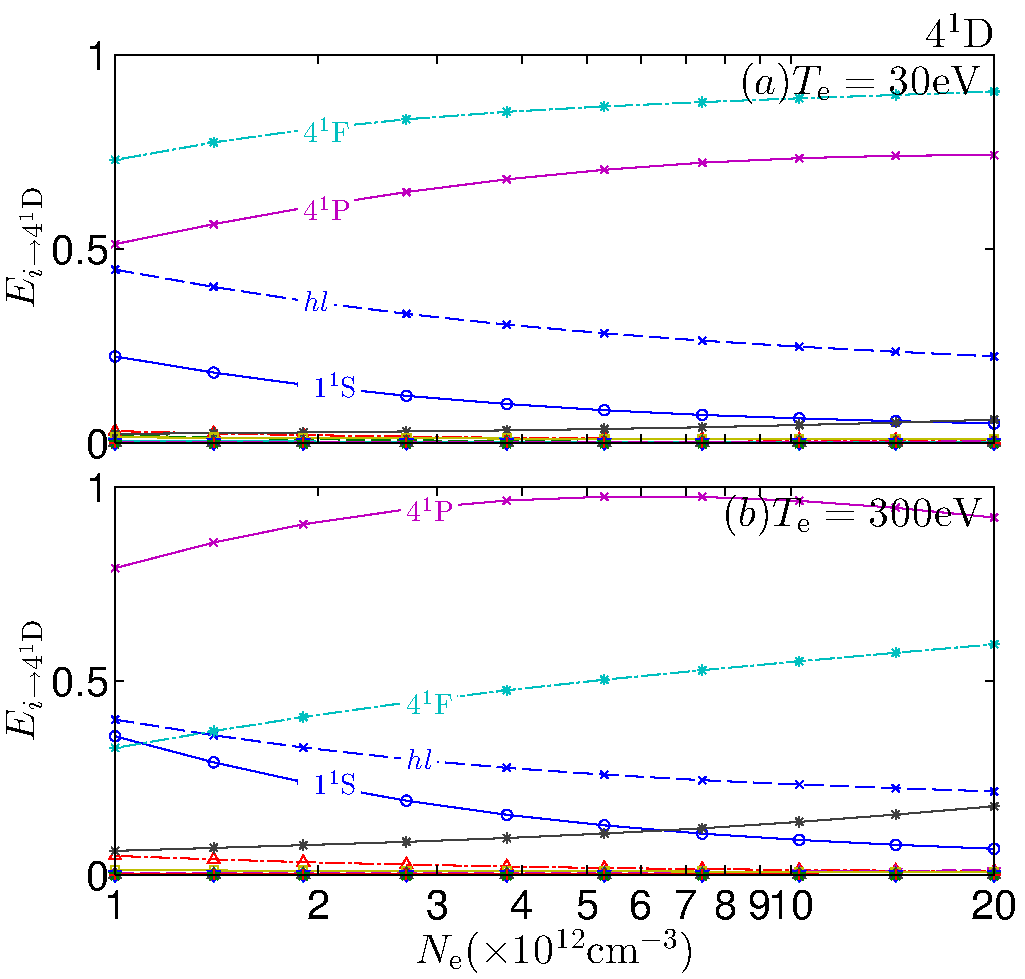
\includegraphics[width=0.6\textwidth]{41D-error-propagation-coefficient.pdf}
  \caption{氦原子 $4^1{\rm D}$ 能级产生过程的速率系数不确定性传递函数}
  \label{fig:chap03:41D-error-propgation-function}
\end{figure}


以 $4^1{\rm D}$ 能级为例,其产生过程的速率系数不确定性传递函数在不同 $T_{\rm e}$ 条件下随电子密度的变化结果在图 \ref{fig:chap03:41D-error-propgation-function} 中画出。在 $T_{\rm e}=30\,{\rm eV}$ 时,来自相同主量子数的相邻能级($4^1{\rm F}$ 和 $4^1{\rm P}$)跃迁产生速率系数不确定性的传递函数随着电子密度的增大而增长,$4^1{\rm F}$ 能级的跃迁速率系数不确定性传递函数甚至会达到 $1$,这意味着 $4^1{\rm F}\to 4^1{\rm D}$ 过程速率系数的不确定性会以相同的量级体现在 $4^1{\rm D}$ 粒子数密度的计算结果上。高能级 $hl$ 与基态能级的不确定性传递函数分别低于 $0.5$ 和 $0.2$,并且随着电子密度的增大而减弱。当电子温度较高时,$4^1{\rm D}$ 各产生过程的速率系数不确定性传递函数具有与电子温度较低时相同的趋势,不过来自 $4^1{\rm F}$ 能级过程的速率系数不确定性传递函数降低到了 $0.5$ 左右,而来自 $4^1{\rm P}$ 过程的速率系数不确定性传递函数则增长到了 $1$ 左右。

\begin{figure}%[H]
  \centering
  \begin{overpic}[width=0.6\textwidth]{41D-error-propagation.pdf}
    \put(-3,16){\rotatebox{90}{\mbox{\colorbox{white}{相对误差 ($\%$)}}}}
    \put(-3,58){\rotatebox{90}{\mbox{\colorbox{white}{相对误差 ($\%$)}}}}
  \end{overpic}
%  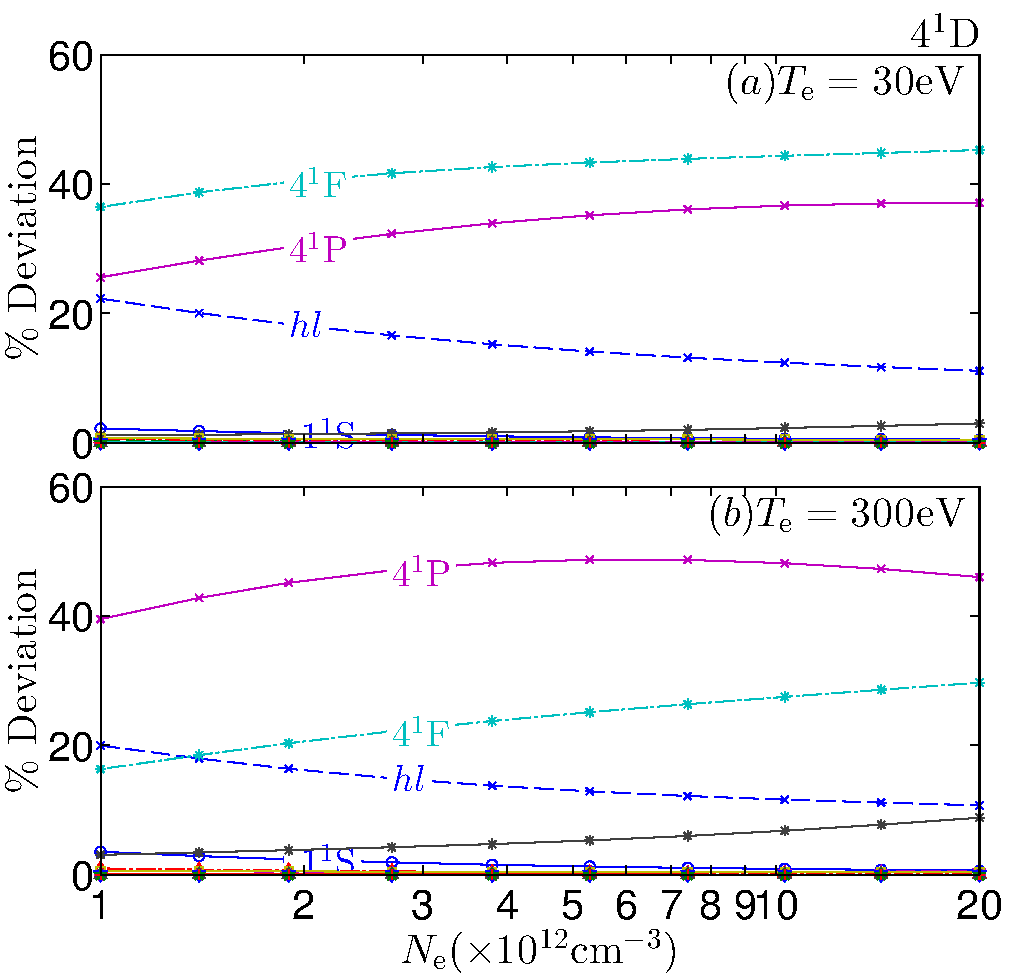
\includegraphics[width=0.6\textwidth]{41D-error-propagation.pdf}
  \caption{氦原子 $4^1{\rm D}$ 能级产生过程的不确定性传递结果}
  \label{fig:chap03:41D-error-propgation-result}
\end{figure}

如图 \ref{fig:chap03:41D-error-propgation-result} 所示,以表 \ref{tab:chap03:rate-uncertainty} 所列各过程的速率系数不确定性为原始数据,分别计算了这些速率系数的不确定性所引起的碰撞辐射模型对 $4^1{\rm D}$ 能级数密度的计算相对误差。由于基态激发速率系数的精度较高,其激发过程的速率系数误差影响可以忽略,而高能级 $hl$ 的速率系数总影响在低于 $20\%$ 的范围内,考虑到这是 $n\ge5$ 的众多能级的总贡献,当只有来自 $n\ge5$ 单一能级的反应过程速率系数具有不确定性时,或这些能级的不确定性均具有不确定性,但不同过程存在正负误差时,高能级产生过程的速率系数不确定性影响可以相互抵消。

在温度较低时,来自相邻能级 $4^1{\rm P}$ 和 $4^1{\rm F}$ 的产生过程速率系数均会带来约 $40\%$ 的相对误差;当温度较高时,$4^1{\rm P}$ 起始过程带来的影响会增加到 $40\%$ 以上,$4^1{\rm F}$ 的影响会降低,但仍保持在 $20\%$ 上下的范围。这说明碰撞辐射模型对相同主量子数能级粒子之间的数密度重新分配过程的速率系数要求很高,但由于实验和理论上的限制,这些速率系数的不确定性精度受到限制\cite{Bray2000:He-data,Delabie2010:consistency},要提高碰撞辐射模型的计算精度,在速率系数的实验、理论上仍需进一步积累\cite{Summers:IAEAdatarequirement}。

由于碰撞辐射模型中多种粒子复杂的反应过程相互耦合,目前尚无手段对反应速率系数不确定性到激发态粒子数密度计算误差的传递进行简洁而有效的计算。前面提到,Y. Andrew 等人\cite{Andrew2000PPCFSensitivity}采用扰动法,将某反应速率系数进行扰动后,重新对碰撞辐射模型进行计算,以获得对速率系数所做的扰动带来的影响。这种对每个速率系数进行扰动并在不同的 $T_{\rm e}$ 和 $N_{\rm e}$ 组合条件下重新解反应速率方程的过程繁复耗时,且不直观,物理意义不明确。我们引入的不确定性传递函数可以直观的体现感兴趣过程的速率系数不确定性到粒子数密度计算结果的影响,且物理意义明确。有助于快速定位对碰撞辐射模型计算产生主要影响的反应过程,并对此做出相应的分析和处理。

另外,通过附录 \ref{appendix:error-propagate} 给出的结果,还可以分析如 ${\rm He}^+$ 复合至基态能级 $1^1{\rm S}$ 的速率系数不确定性通过两次反应过程对如 $n=4$ 的普通激发态能级数密度产生影响的不确定性传递函数,甚至是通过三级或多级反应过程的不确定性传递函数。

\subsection{碰撞辐射模型中包含的能级对计算结果影响的研究}
\label{sec:chap03:maxn-in-crm}

碰撞辐射模型中包含的能级与反应过程的多少对感兴趣能级粒子数密度的计算会产生影响。我们知道,由于反应过程速率系数不确定性的存在,模型包含更多数目的能级和反应过程并不能如以前人们所预期的那样可以得到更高精度的粒子数密度计算结果。本节主要研究包含到最高能级主量子数 $\max n$ 至什么程度即可以满足对计算精度的要求。

由于氦原子 $n\le4$ 能级的电子碰撞电离与它们之间的跃迁截面数据具有较高的精度,对于 SUNIST 参数下的氦等离子体,我们分别计算在碰撞辐射模型最高包含至 $\max n=5, 6, 7 \cdots$ 时能级粒子数密度的计算结果与最高包含至 $\max n-1$ 时计算结果的相对误差:
\begin{equation}
\Delta N_i^{\max n}=100\%\times\frac{N_i^{\max n}-N_i^{\max n-1}}{N_i^{\max n-1}}
\label{eq:chap03:rel-diff-maxn}
\end{equation}
其中,$N_i^{\max n}$ 与 $N_i^{\max n-1}$ 分别为碰撞辐射模型包含最高至主量子数为 $\max n$ 和  $\max n-1$ 时的 $i$ 能级粒子数密度计算结果。

\begin{figure}%[H]
    \centering
    \begin{subfigure}{0.47\textwidth}
        %\begin{overpic}[width=\textwidth]{levelabun-13-41S-Ne5_0E12-ss-reldiff-manx4to7.pdf}
        %    \put(-2,40){\rotatebox{90}{\colorbox{white}{$\Delta_{N_{4^1{\rm S}}}^{\max n}$ ($\%$)}}}
        %\end{overpic}
        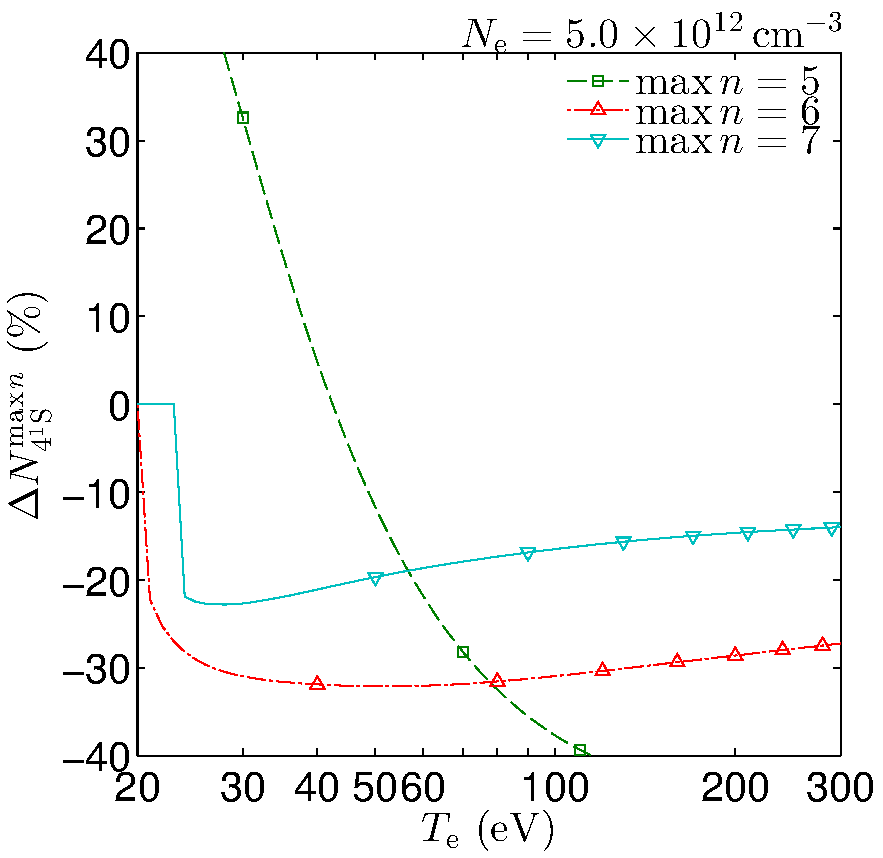
\includegraphics[width=\textwidth]{levelabun-13-41S-Ne5_0E12-ss-reldiff-manx4to7.pdf}
        \caption{随 $T_{\rm e}$ 的变化}%
        \label{fig:chap03:41S-levelabun-reldiff:1}
    \end{subfigure}
    %\hspace{0.05\textwidth}
    \begin{subfigure}{0.47\columnwidth}
        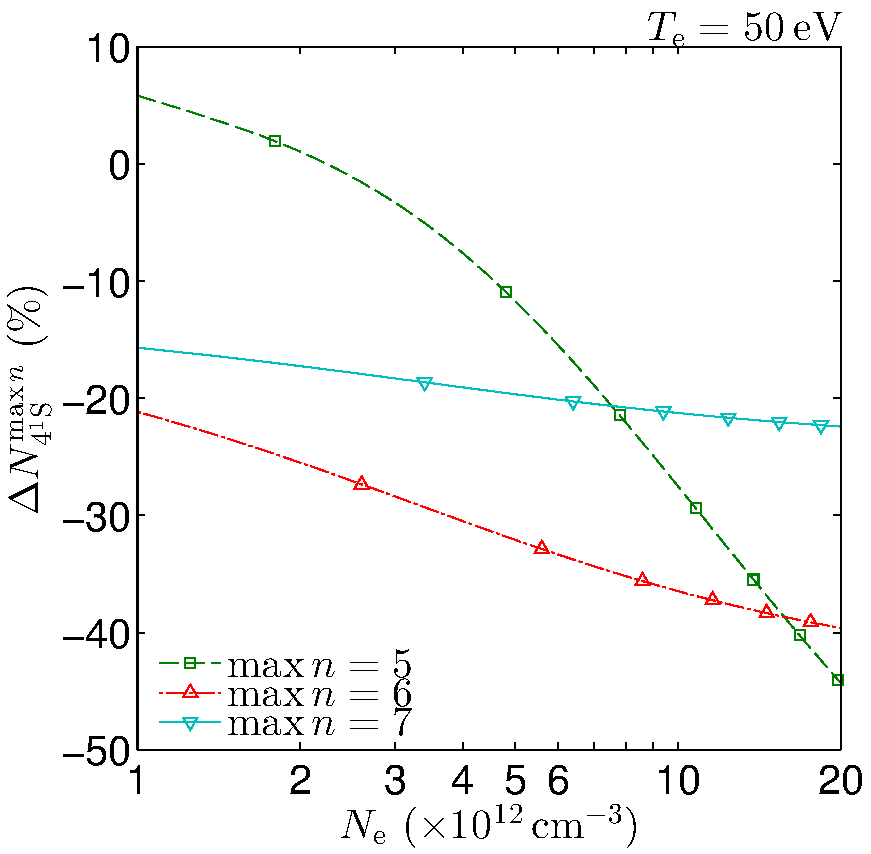
\includegraphics[width=\columnwidth]{levelabun-13-41S-Te50-ss-reldiff-manx4to7.pdf}
        \caption{随 $N_{\rm e}$ 的变化}%
        \label{fig:chap03:41S-levelabun-reldiff:2}
    \end{subfigure}
    \caption{包含至不同最高主量子数能级时,氦原子 $4^1{\rm S}$ 能级数密度计算的相对误差。}%
    \label{fig:chap03:41S-levelabun-reldiff}
\end{figure}

\begin{figure}%[H]
  \centering
  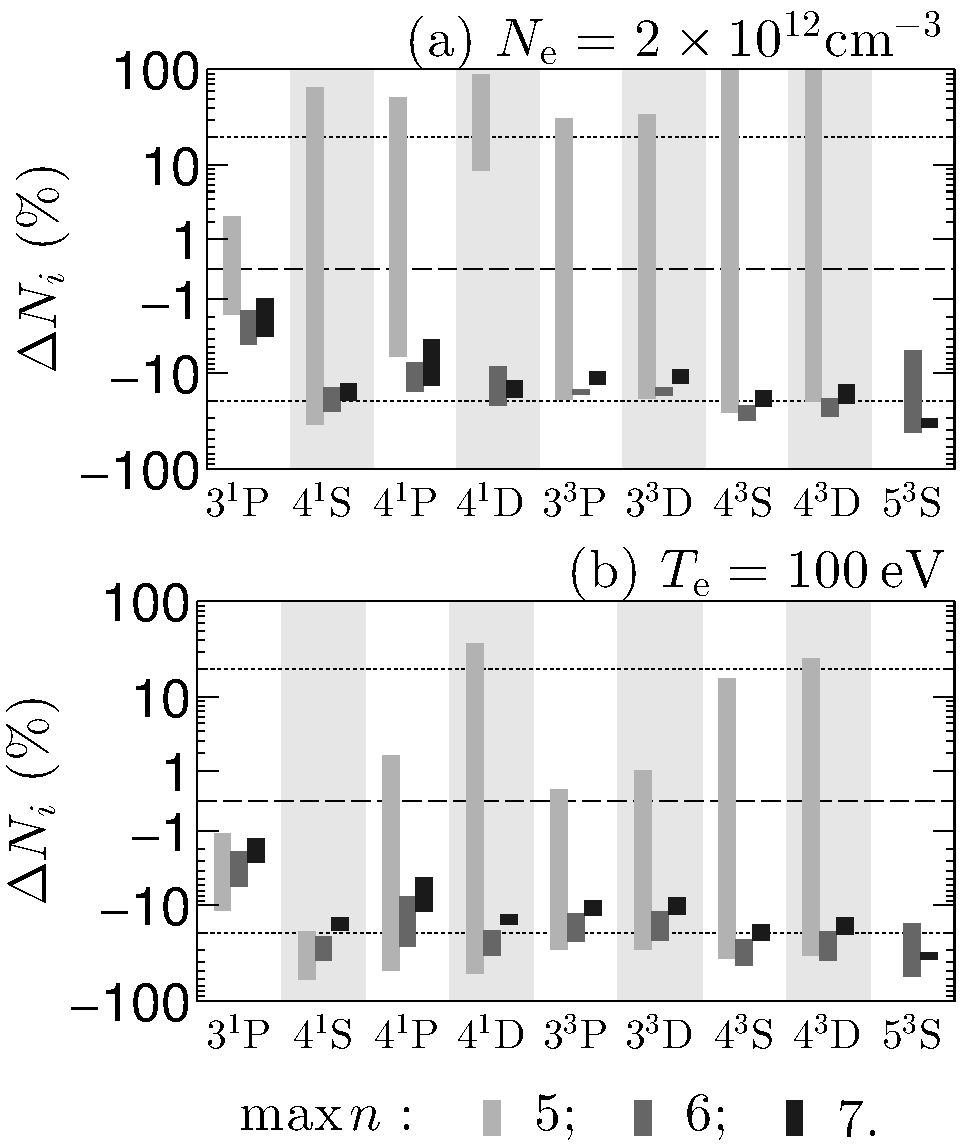
\includegraphics[width=0.7\textwidth]{levelabun-reldiff-maxn5to7-helines.pdf}
  \caption{包含至不同最高主量子数能级时,$n\leq4$ 能级的相对计算误差范围。图片来自 \onlinecite{xie:wlxb}。}
  \label{fig:chap03:levelabun-reldiff-all}
\end{figure}

以 $4^1{\rm S}$ 能级为例,图 \ref{fig:chap03:41S-levelabun-reldiff} 所示为该能级在碰撞辐射模型最高包含至不同 $\max n$ 时,计算结果的相对误差随电子温度或电子密度的变化。由图 \ref{fig:chap03:41S-levelabun-reldiff:1} 可见,随着 $T_{\rm e}$ 的升高,$\Delta N_{4^1{\rm S}}^{\max n=5}$ 自 $+40\%$ 急剧下降到 $-40\%$,虽然在 $T_{\rm e}\sim40\,{\rm eV}$ 附近,对于 $\max n=5$ 的碰撞辐射模型计算相对误差接近零,但总体来讲 $\max n=5$ 的碰撞辐射模型计算结果是不可接受的。$\Delta N_{4^1{\rm S}}^{\max n=5}$ 随 $N_{\rm e}$ 增长的变化规律类似(图 \ref{fig:chap03:41S-levelabun-reldiff:2}),当 $N_{\rm e}$ 自 $1\times10^{12}\,{\rm cm}^{-3}$ 至 $2\times10^{13}\,{\rm cm}^{-3}$ 变化时,$\Delta N_{4^1{\rm S}}^{\max n=5}$ 从 $+8\%$ 降低至 $-40\%$。当 $\max n$ 分别取 $6$ 和 $7$ 时,$\Delta N_{4^1{\rm S}}^{\max n=6}$ 和 $\Delta N_{4^1{\rm S}}^{\max n=7}$ 具有相同的变化趋势:随 $T_{\rm e}$ 的升高,计算误差短暂急剧上升之后,趋于平缓并有所下降(图 \ref{fig:chap03:41S-levelabun-reldiff:1});随着 $N_{\rm e}$ 的增长,计算误差增加(图 \ref{fig:chap03:41S-levelabun-reldiff:2})。$\Delta N_{4^1{\rm S}}^{\max n=6}$ 具有较大的误差数值,而 $\Delta N_{4^1{\rm S}}^{\max n=7}$ 在 $20\%$ 的相对误差范围内。

由图 \ref{fig:chap03:41S-levelabun-reldiff} 可以计算在特定的 $T_{\rm e}$ 或 $N_{\rm e}$ 参数下,各能级的计算误差 $\Delta_i^{\max n}$ 随另外一个参数变化时的总体范围,SUNIST 氦原子发射光谱实验(第 \ref{sec:chap04:sunist-spec-measurements} 节)所测量的氦原子谱线上能级计算结果如图 $\ref{fig:chap03:levelabun-reldiff-all}$ 所示。以此,我们可以得出在适用的等离子体参数范围内,碰撞辐射模型中最高包含至主量子数能级达什么程度时,其计算结果是可以接受的。当最高包含至 $\max n=5$ 时,计算结果的相对误差范围较大,甚至可达 $100\%$ 的范围,这是不可接受的;当最高包含至$\max n=6$ 时,计算误差范围开始缩小,但是对于用来进行谱线比诊断的 $n=4$ 能级粒子数的计算相对误差还是会超过 $20\%$;当 $\max n=7$ 时,除 $5^3{\rm S}$ 能级外的各能级粒子数计算结果的相对误差可以控制在 $20\%$ 以内。根据第 \ref{sec:chap04:uncertainty-transport} 节的分析,当 $n=4$ 能级与相邻能级之间电子碰撞跃迁速率系数存在不确定性时,其引起的能级粒子数密度相对计算误差即可达 $40\%$,由此,可以认为碰撞辐射模型中包含至最高主量子数为 $\max n=7$ 的能级时,计算结果已经可以接受,这与第 \ref{sec:chap03:level-selection} 节的处理相符。

图 \ref{fig:chap03:levelabun-reldiff-all} 还显示,当包含至更高能级时,粒子数的计算相对误差为负值。这是因为对 $n\ge 8$ 能级的舍弃切断了较低能级碰撞激发和电离的路径\cite{Fujimoto1979-HeCR},则碰撞辐射模型的计算中,包含至更高主量子数能级的能级数密度计算结果具有更低的值。%图 \ref{fig:chap03:levelabun-reldiff-all} 还显示
另外,在碰撞辐射模型取不同的 $\max n$ 时,各能级的数密度计算值具有强相关性。

\subsection{对谱线比计算结果影响的估计}

本文主要是利用碰撞辐射模型对氦原子谱线的相对强度进行等离子体 $T_{\rm e}$ 和 $N_{\rm e}$ 的诊断,通过下面的推导可以对碰撞辐射模型激发态数密度计算的不确定度对谱线强度比引起的影响进行估计。模型计算的来自 $q\to p$ 与 $j\to i$ 跃迁的两谱线强度比为:
\begin{equation}
\label{eq:chap03:lineratio-error}
r^{\rm mod}=\frac{A_{q\to p}n_q}{A_{j\to i}n_j},
\end{equation}
其中,爱因斯坦系数 $A_{q\to p}$ 与 $A_{j\to i}$ 的精度可以保证。则谱线比误差的主要来自模型对高能级数密度 $n_q$ 与 $n_j$ 的计算,可以写为\cite{burgos2012:PoP}:
\begin{equation}
\label{eq:chap03:ErrorModeledLineratio}
\begin{aligned}
\delta_r^{\rm mod} = & \pm r^{\rm mod}\\
& \times\sqrt{\left(\frac{\delta_{n_q}}{n_q}\right)^2 + \left(\frac{\delta_{n_j}}{n_j}\right)^2 - 2\gamma_{qj}\frac{\delta_{n_q}\delta_{n_j}}{n_qn_j}},
\end{aligned}
\end{equation}
其中,$\gamma_{qj}$ 代表 $q$ 与 $j$ 能级数密度的相关系数。假设$\delta_{n_q}/n_q\approx \delta_{n_j}/n_j=\delta_n/n$,则式 (\ref{eq:chap03:ErrorModeledLineratio}) 可以简化为:
\begin{equation}
\label{eq:chap03:SimpleErrorModeledLineratio}
r^{\rm mod} \approx\pm r^{\rm mod} \times \sqrt{2\left(\frac{\delta_n}{n}\right)^2(1-\gamma_{qj})},
\end{equation}
从式 (\ref{eq:chap03:SimpleErrorModeledLineratio}) 可以看出,对于激发态数密度具有高相关性的两条谱线,即 $\gamma_{qj}\sim 1$ 时,碰撞辐射模型计算的能级数密度误差可以抵消。

自旋单重态能级数密度之间与自旋三重态能级数密度之间具有高相关性,可以忽略单重态能级谱线之间与三重态能级谱线之间强度比的模型计算误差。单重态能级谱线强度与三重态能级谱线强度分别主要对 $T_{\rm e}$ 和 $N_{\rm e}$ 敏感,这可以解释图 \ref{fig:chap04:RelLevelabunAt3Times} 中显示的单重态与三重态能级数密度的碰撞辐射模型计算结果随 $T_{\rm e}$ 和 $N_{\rm e}$ 参数呈现出的集体变化趋势。由图 $\ref{fig:chap03:levelabun-reldiff-all}$ 可见,对于 $n=4$ 激发态各能级数密度的计算之间具有强的相关性,且相对计算误差小于 $20\%$,所以本文碰撞辐射模型的谱线比计算结果误差应远小于 $20\%$。

\section{SUNIST 等离子体谱线比诊断方法的建立}
\label{sec:chap03:lineratio-method}

\subsection{谱线强度比的选择}
\label{sec:chap03:lineratio-selection}

一般地,在氦原子发射光谱诊断实验中,人们选择来自 $n=3$ 激发态能级的三条谱线\pozhehao $667.8\,{\rm nm}\,(3^1{\rm D}-2^1{\rm P})$、$706.5\,{\rm nm}\,(3^3{\rm S}-2^3{\rm P})$ 和 $728.1\,{\rm nm}\,(3^1{\rm S}-2^1{\rm P})$ \pozhehao 的强度比进行 $T_{\rm e}$ 和 $N_{\rm e}$ 的诊断。但是,对于较高电子密度($N_{\rm e}>10^{13}\,{\rm cm}^{-3}$)的等离子体,$706.5\,{\rm nm}\,(3^3{\rm S}-2^3{\rm P})$ 谱线辐射在等离子体中会被强烈再吸收\cite{boivin2001,Boivin2007},此时氦等离子体实际的谱线测量结果与碰撞辐射模型也存在着明显的差别\cite{Schweer1992174,Brosda1993:Thesis,Sasaki:NIFS:DATA:346}。

SUNIST 等离子体对 $501.6\,{\rm nm}\,(3^1{\rm P}-2^1{\rm S})$、$396.5\,{\rm nm}\,(4^1{\rm P}-2^1{\rm S})$ 与 $388.9\,{\rm nm}\,(3^3{\rm P}-2^3{\rm S})$ 具有明显的再吸收作用(第 \ref{sec:chap04:lineratio-ne-te} 节),则这三条谱线也不适合用来进行谱线的辐射诊断,而谱线 $412.1\,{\rm nm}\,(5^3{\rm S}-2^3{\rm P})$ 来自 $n=5$ 壳层,其强度相对 $n=3$ 和 $n=4$ 壳层的谱线要弱。所以,本文在 $504.8\,{\rm nm}\,(4^1{\rm S}-2^1{\rm P})$、$492.2\,{\rm nm}\,(4^1{\rm D}-2^1{\rm P})$、$587.6\,{\rm nm}\,(3^3{\rm D}-2^3{\rm P})$、$471.3\,{\rm nm}\,(4^3{\rm S}-2^3{\rm P})$ 和 $447.1\,{\rm nm}\,(4^3{\rm D}-2^3{\rm P})$ 五条谱线中挑取分别来自不同自旋系统的三条谱线,建立同时进行 $T_{\rm e}$ 和 $N_{\rm e}$ 诊断的谱线比法。

\begin{figure}
  \centering
  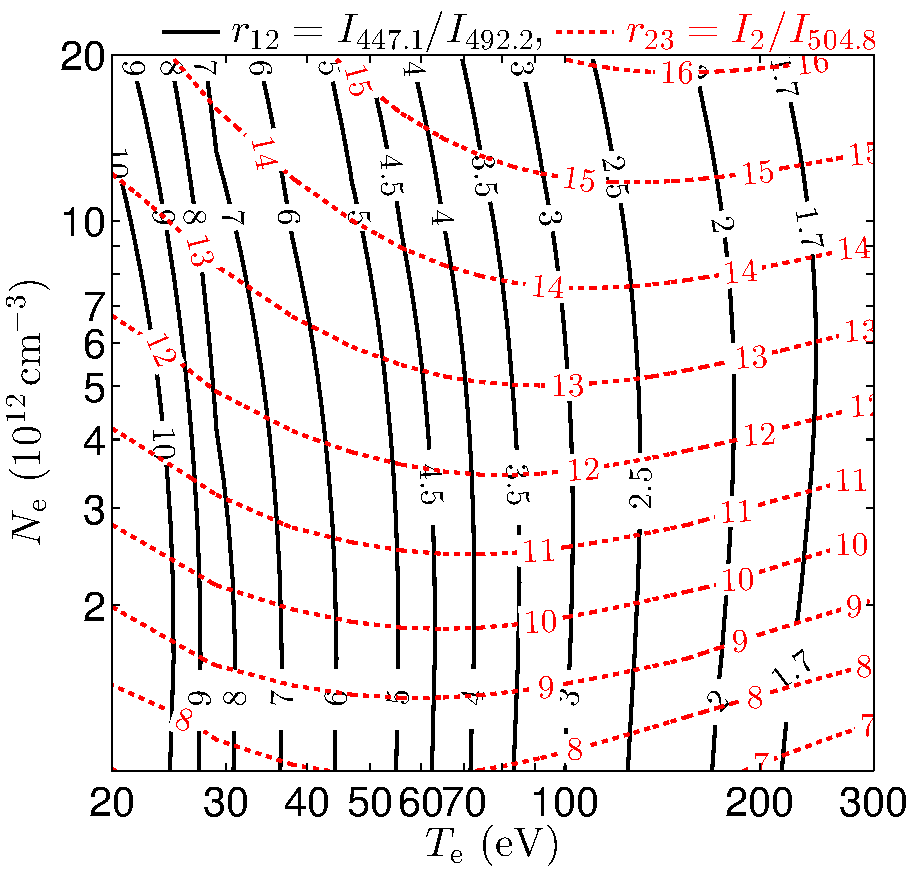
\includegraphics[width=0.6\textwidth]{1-9to7-7to5-getTeNe-lineratio.pdf}
  \caption{SUNIST 上使用的来自 $n=4$ 激发态能级的三条谱线的谱线比。图片来自 \onlinecite{xie:wlxb}。}
  \label{fig:chap03:getTeNe-lineratio}
\end{figure}

\begin{figure}
  \centering
  \begin{subfigure}{0.45\textwidth}
    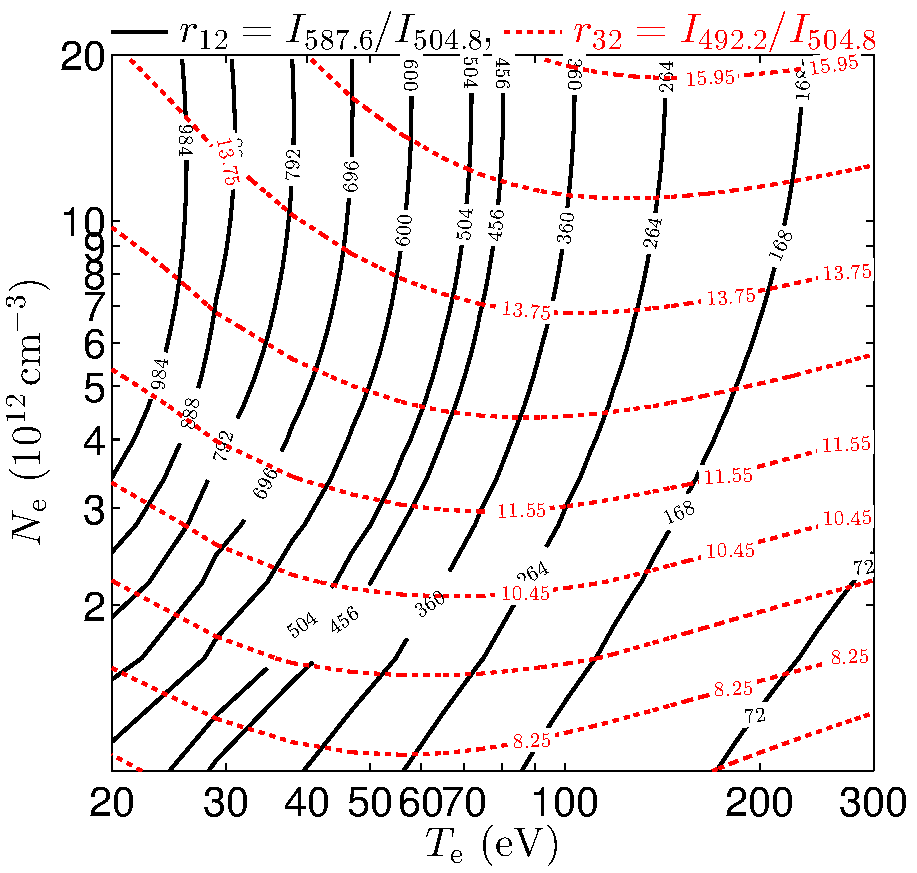
\includegraphics[width=\textwidth]{1-4to5-7to5-getTeNe-lineratio.pdf}
    \caption{}
    \label{fig:chap03:lineratio-backup:1}
  \end{subfigure}
  \hspace{0.05\textwidth}
  \begin{subfigure}{0.45\textwidth}
    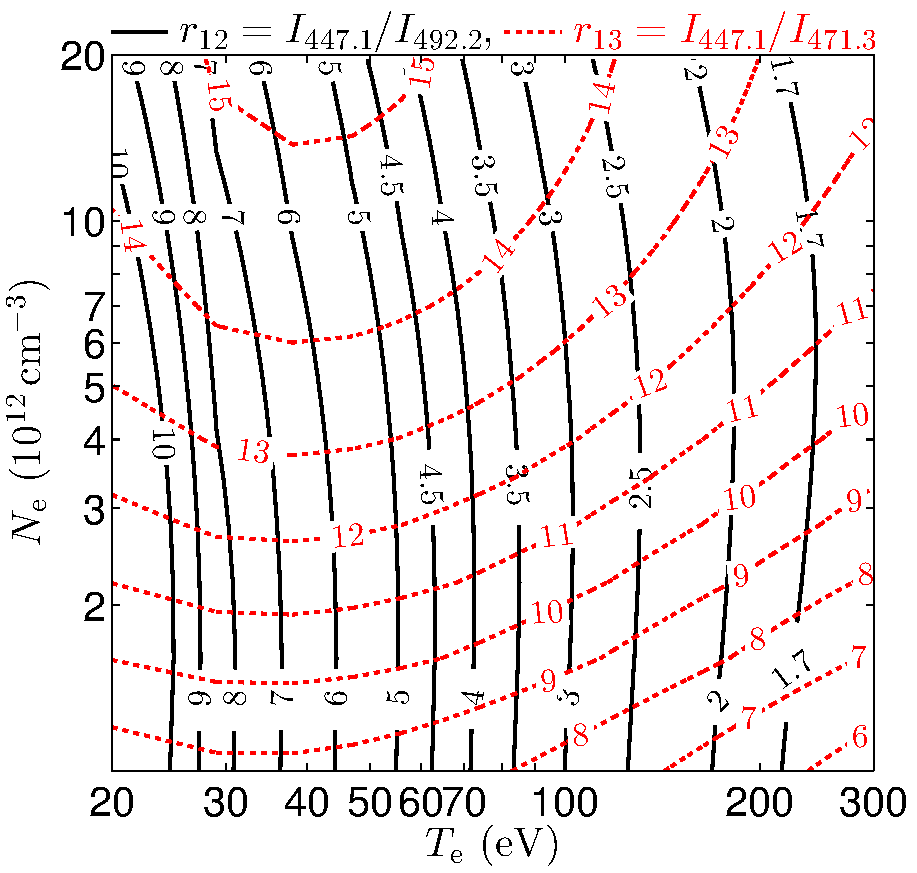
\includegraphics[width=\textwidth]{1-9to8-9to7-getTeNe-lineratio.pdf}
    \caption{}
    \label{fig:chap03:lineratio-backup:2}
  \end{subfigure}
  \caption{SUNIST 上可用来做谱线比诊断的其他谱线比备选方案}
  \label{fig:chap03:lineratio-backup}
\end{figure}

图 \ref{fig:chap03:getTeNe-lineratio} 与 图 \ref{fig:chap03:lineratio-backup} 分别显示本文所使用的谱线比计算结果与可以用来进行谱线比诊断的备选谱线比方案。其中,图 \ref{fig:chap03:lineratio-backup:1} 所显示的谱线比中,$T_{\rm e}$ 敏感谱线比 $r_{12}=I_{587.6}/I_{504.8}$ 在 $N_{\rm e}<5\times10^{12}\,{\rm cm}^{-3}$ 时,显示出与 $N_{\rm e}$ 较强的函数关系,同时此谱线比分别来自 $n=3$ 和 $n=4$ 的两激发态能级粒子,其强度差距悬殊,不利于谱线比法的应用。图 \ref{fig:chap03:lineratio-backup:2} 的备选方案中,$N_{\rm e}$ 敏感谱线比 $r_{13}=I_{447.1}/I_{471.3}$ 在低温高密度($T_{\rm e}<100\,{\rm eV}$,$N_{\rm e}>5\times10^{12}\,{\rm cm}^{-3}$)区,对电子温度的诊断会出现重复取值的问题。图 \ref{fig:chap03:getTeNe-lineratio} 显示的谱线比方案,谱线强度之间的比值范围合适,且电子温度和密度敏感的谱线比也显示出了优越的独立于另外一个参数的性质。

\subsection{谱线比法确定等离子体参数的过程}

\begin{figure}
  \centering
  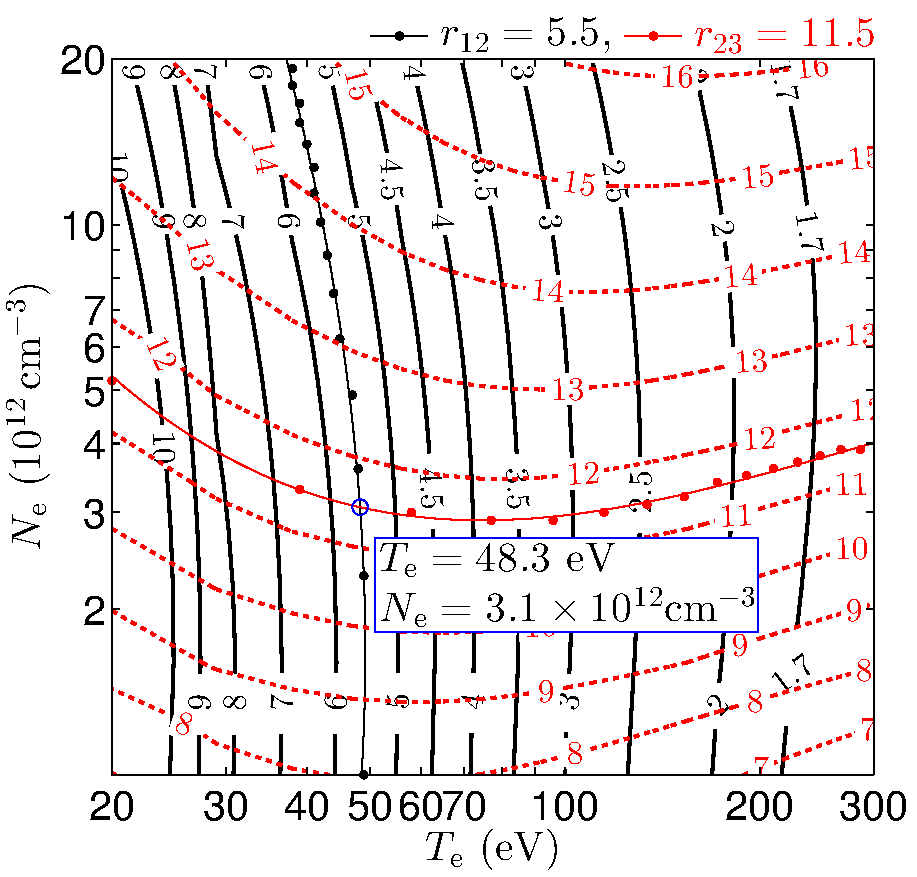
\includegraphics[width=0.6\textwidth]{5-9to7-7to5-getTeNe-crosspoint.pdf}
  \caption{谱线比法确定 $T_{\rm e}$ 和 $N_{\rm e}$ 参数}
  \label{fig:chap03:getTeNe-cross-pnt}
\end{figure}

以图 \ref{fig:chap03:getTeNe-lineratio} 中所示的谱线比计算结果为基础,图 \ref{fig:chap03:getTeNe-cross-pnt} 中以谱线比测量结果为 $r_{12}=5.5$,$r_{23}=11.5$ 时为例,显示了同时确定 $T_{\rm e}$ 和 $N_{\rm e}$ 的方法与过程。

1)寻点

在 $T_{\rm e}$、$N_{\rm e}$ 二维空间上的 $r_{12}(T_{\rm e},N_{\rm e})$ 与 $r_{23}(T_{\rm e},N_{\rm e})$ 计算值内,分别寻找 $r_{12}=5.5$ 和 $r_{23}=11.5$ 的 $(T_{\rm e}, N_{\rm e})$ 点,如图 \ref{fig:chap03:getTeNe-cross-pnt} 所示。

2)拟合

对于 $T_{\rm e}$ 敏感谱线比,将寻找到的一系列 $(T_{\rm e}, N_{\rm e})$ 寻点取值结果用下面的多项式进行拟合:
\begin{equation}
    \label{eq:chap03:getTeNe:r12-fit}
    T_{\rm e} = \sum_{i=0}^{3}C_{i}N_{\rm e}^{i}
\end{equation}
得到 $C_i$ 系数。

对于 $N_{\rm e}$ 敏感谱线比,则将 $(T_{\rm e}, N_{\rm e})$ 取值系里用下面的多项式拟合:
\begin{equation}
    \label{eq:chap03:getTeNe:r32-fit}
    N_{\rm e} = \sum_{j=0}^{3}C_{j}T_{\rm e}^{j}
\end{equation}
得到 $C_j$ 系数。多项式曲线拟合结果在图 \ref{fig:chap03:getTeNe-cross-pnt} 中给出。

3)求交点

联立方程 (\ref{eq:chap03:getTeNe:r12-fit}) 与 (\ref{eq:chap03:getTeNe:r32-fit}),求出其交点,则可以同时得到此交点的 $T_{e}$ 和 $N_{\rm e}$ 值,如图 \ref{fig:chap03:getTeNe-cross-pnt} 所示,当 $r_{12}=5.5$ 和 $r_{23}=11.5$ 时,等离子体的电子温度和电子密度参数分别为 $48.3\,{\rm eV}$ 和 $3.1\times10^{12}\,{\rm cm}^{-3}$。

\subsection{实际谱线比测量误差到 $T_{\rm e}$ 和 $N_{\rm e}$ 诊断误差传递的研究}
\label{sec:chap03:lineratio-error-to-result-error}

\begin{figure}%[H]
  \centering
  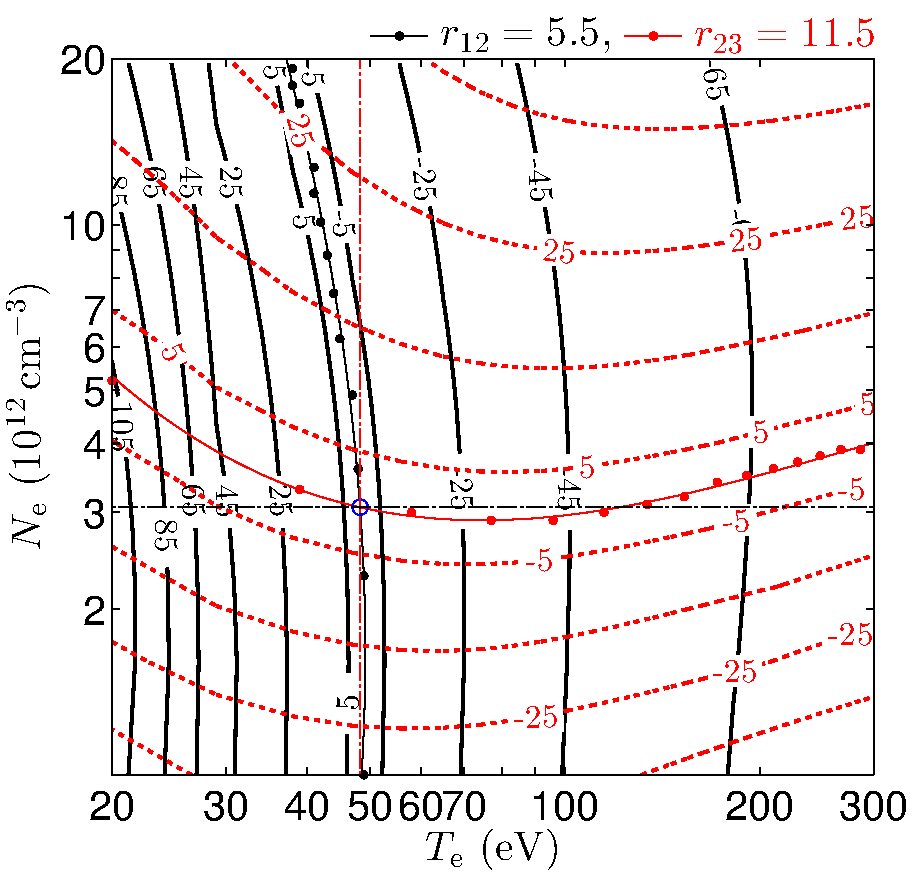
\includegraphics[width=0.6\textwidth]{6-9to7-7to5-getTeNe-errorroute.pdf}
  \caption{谱线比测量误差至 $T_{\rm e}$ 和 $N_{\rm e}$ 诊断误差传递的计算路径,其中谱线比等高线已经转换为了相对测量百分比误差等高线。}
  \label{fig:chap03:getTeNe-error-route}
\end{figure}

图 \ref{fig:chap03:getTeNe-cross-pnt} 中给出了谱线比法确定 $T_{\rm e}$ 和 $N_{\rm e}$ 的方法和过程,为了研究谱线比实验测量误差至 $T_{\rm e}$ 和 $N_{\rm e}$ 诊断结果误差的传递,在图 \ref{fig:chap03:getTeNe-error-route} 中,将谱线比等高线转换为相对图 \ref{fig:chap03:getTeNe-cross-pnt} 中示例谱线比的测量误差等高线。

对于电子温度 $T_{\rm e}$ 敏感谱线比 $r_{12}=I_{447.1}/I_{492.2}$,J.M.M. Burgos\cite{burgos2012:PoP} 计算了当电子密度 $N_{\rm e}$ 为固定值 $1.0\times10^{12}\,{\rm cm}^{-3}$ 时谱线比测量误差在不同 $T_{\rm e}$ 时对 $T_{\rm e}$ 诊断带来的误差,对应到图 \ref{fig:chap03:getTeNe-cross-pnt} 所示的谱线比法,则为 $N_{\rm e}=3.1\times10^{12}\,{\rm cm}^{-3}$ 时的计算路径,即图 \ref{fig:chap03:getTeNe-error-route} 中所示水平点画线。然而,仅通过 $T_{\rm e}$ 敏感谱线比是无法确定电子密度 $N_{\rm e}$ 参数的,在计算 $T_{\rm e}$ 敏感谱线比测量误差对 $T_{\rm e}$ 诊断结果影响时,固定 $N_{\rm e}$ 敏感谱线比值做为前提条件的计算路径是更符合实际情况的,即图 \ref{fig:chap03:getTeNe-error-route} 中所示 $r_{23}=11.5$ 的近似水平拟合实线曲线路径。

\begin{figure}%[H]
  \centering
    \begin{overpic}[width=0.6\textwidth]{7-9to7-7to5-getTeNe-errorpropagation.pdf}
    \put(0,0){\rotatebox{90}{\mbox{\colorbox{white}{\hspace{2em}谱线比误差 ($\%$)\hspace{2em}}}}}
    \put(-2,50){\rotatebox{90}{\mbox{\colorbox{white}{\hspace{2em}谱线比误差 ($\%$)\hspace{2em}}}}}
  \end{overpic}
  %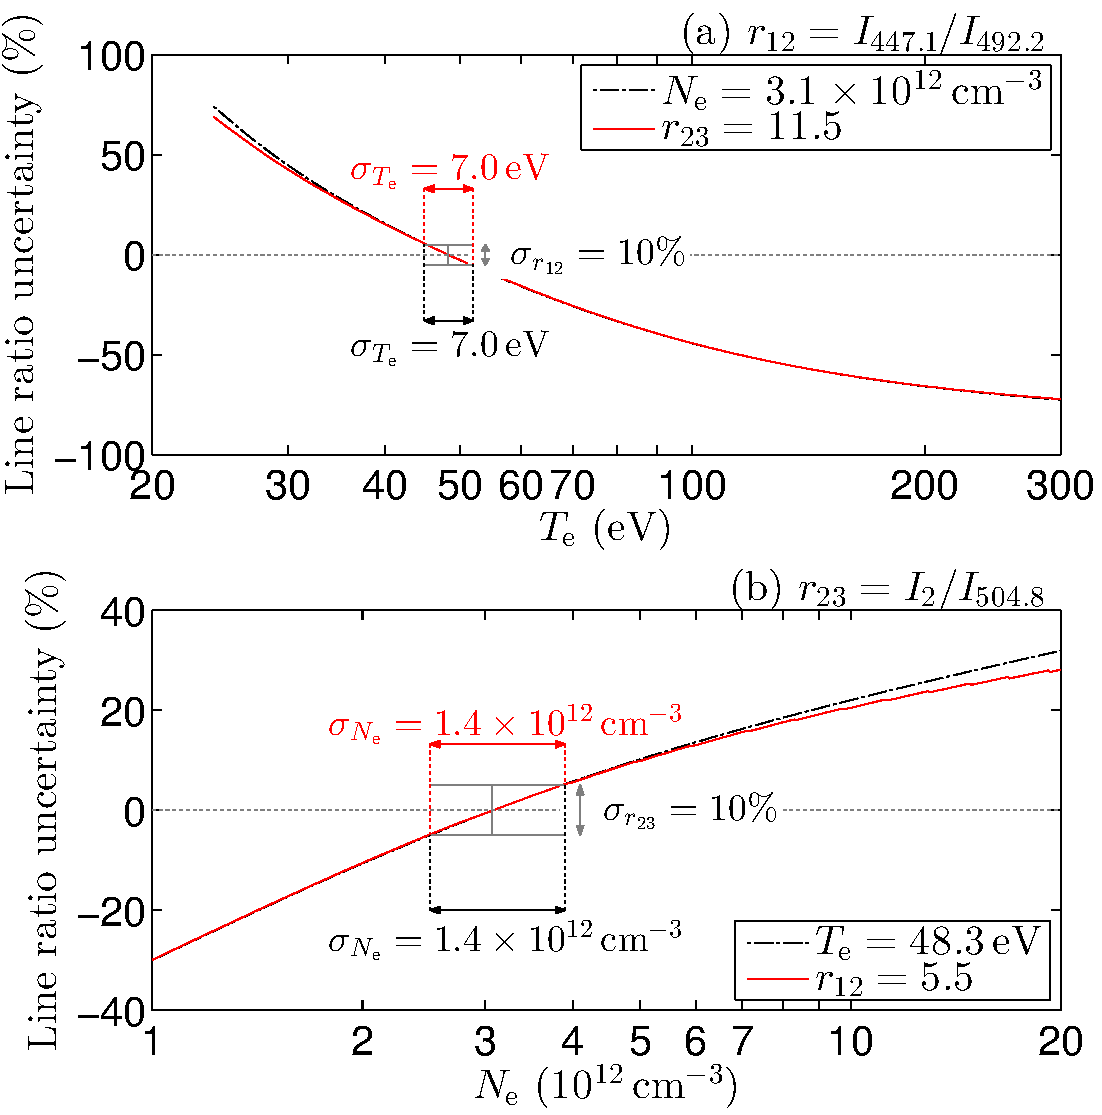
\includegraphics[width=0.6\textwidth]{7-9to7-7to5-getTeNe-errorpropagation.pdf}
  \caption{不同计算路径上的谱线比相对误差与等离子体参数诊断误差示意图。(a):$T_{\rm e}$ 敏感谱线比 $r_{12}$ 在固定 $N_{\rm e}$ 和固定 $r_{23}$ 时的计算路径;(b):$N_{\rm e}$ 敏感谱线比 $r_{23}$ 在固定 $T_{\rm e}$ 和固定 $r_{12}$ 时的计算路径。}
  \label{fig:chap03:getTeNe-errorpropagation}
\end{figure}

沿固定 $N_{\rm e}=3.1\times10^{12}\,{\rm cm}^{-3}$ 和固定 $r_{23}=11.5$ 计算路径的 $T_{\rm e}$ 敏感谱线比相对示例值 $5.5$ 的误差在图 \ref{fig:chap03:getTeNe-errorpropagation}(a) 中画出。由此可以计算出谱线比测量误差 $\sigma_{r_{12}}$ 所对应的 $T_{\rm e}$ 诊断误差值 $\sigma_{T_{\rm e}}$,如图 \ref{fig:chap03:getTeNe-errorpropagation}(a) 所示,当 $T_{\rm e}=48.3\,{\rm eV}$ 时,对于 $10\%$ ($\pm5\%$)的谱线比测量误差,两种不同路径计算的 $\sigma_{T_{\rm e}}$ 均为 $\sim7.0\,{\rm eV}$,因为两不同误差计算路径在此处具有相近的走向(图 \ref{fig:chap03:getTeNe-error-route})。由图 \ref{fig:chap03:getTeNe-errorpropagation}(a) 还可以得到,沿误差计算路径的谱线比误差曲线随 $T_{\rm e}$ 变化的斜率越大,谱线比测量误差引起的 $T_{\rm e}$ 诊断误差越小。

%在 $T_{\rm e}$ 为 $20-30\,{\rm eV}$ 时,两误差计算路径走向差别

\begin{figure}%[H]
  \centering
  \centering
    \begin{overpic}[width=0.6\textwidth]{8-9to7-7to5-getTeNe-errorpropagationscan.pdf}
    \put(0,18){\rotatebox{90}{\mbox{\colorbox{white}{ $\sigma_{T_{\rm e}}/T_{\rm e}$ ($\%$) }}}}
    \put(0,65){\rotatebox{90}{\mbox{\colorbox{white}{ $\sigma_{N_{\rm e}}/N_{\rm e}$ ($\%$) }}}}
  \end{overpic}
  %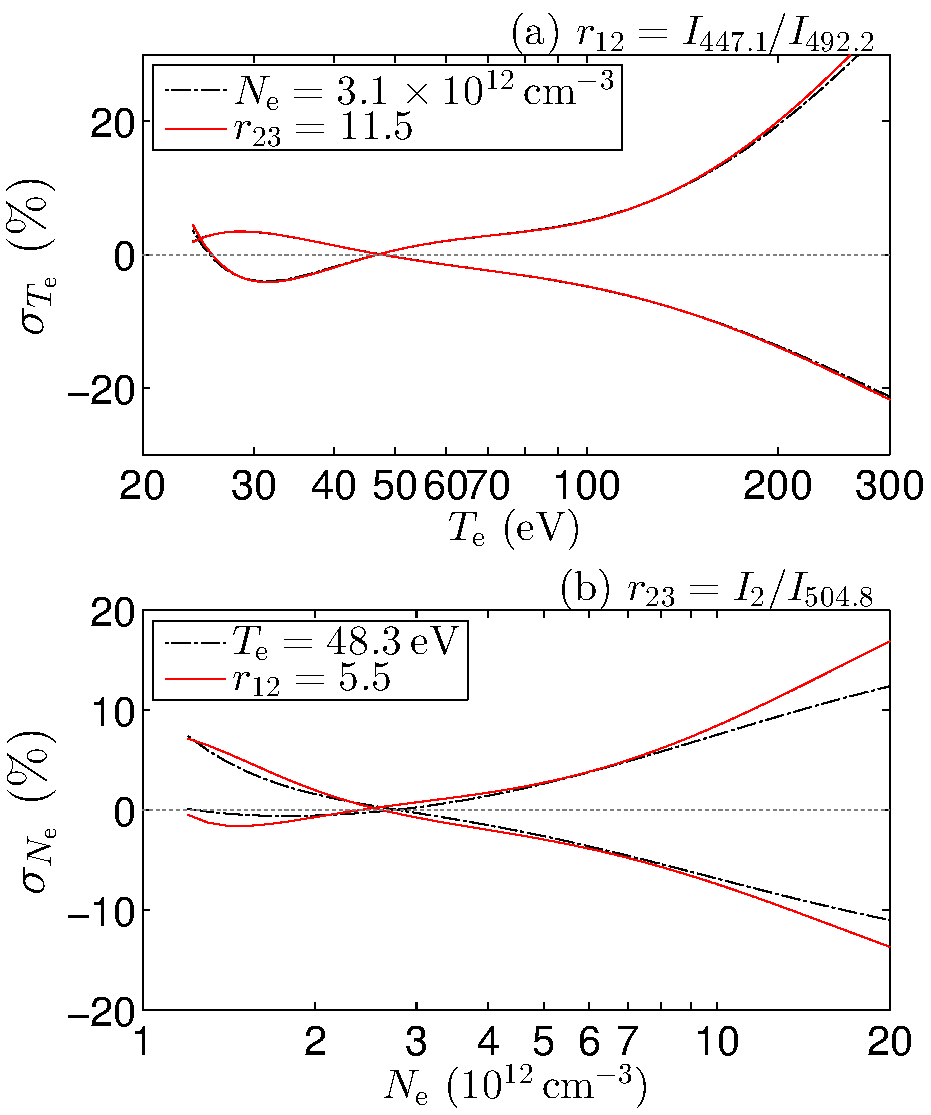
\includegraphics[width=0.6\textwidth]{8-9to7-7to5-getTeNe-errorpropagationscan.pdf}
  \caption{$10\%$ 的谱线比测量误差沿不同计算路径引起的相对诊断误差范围。(a):$\sigma_{T_{\rm e}}/T_{\rm e}$;(b):$\sigma_{N_{\rm e}}/N_{\rm e}$。}
  \label{fig:chap03:getTeNe-errorpropagationscan}
\end{figure}

以图 \ref{fig:chap03:getTeNe-errorpropagation}(a) 所示的计算方法,在不同的 $T_{\rm e}$ 情况下,$10\%$ 的 $r_{12}$ 测量误差沿不同误差计算路径对电子温度诊断的相对误差 $\sigma_{T_{\rm e}}/T_{\rm e}$ 范围曲线在图 \ref{fig:chap03:getTeNe-errorpropagationscan}(a) 中画出。可见,对于 $T_{\rm e}$ 敏感谱线比,当 $T_{\rm e}<100\,{\rm eV}$ 时,$\pm5\%$ 的谱线比测量结果误差所引起的 $T_{\rm e}$ 相对诊断误差范围在 $\pm10\%$ 以内。当 $T_{\rm e}>100\,{\rm eV}$ 时,谱线比法对电子温度的诊断开始对谱线比测量误差变得越来越敏感,对 $T_{\rm e}$ 诊断的相对误差范围会逐步增长至 $\pm20\%$ 以上。两不同误差计算路径之间具有微弱差别,这是因为在感兴趣的 $T_{\rm e}$ 范围内两路径的走向具有相近的走势,且与 $r_{12}$ 等高线的夹角也相近(图 \ref{fig:chap03:getTeNe-error-route})。

对于电子密度 $N_{\rm e}$ 敏感谱线比 $r_{23}=I_{492.2}/I_{504.8}$,固定 $T_{\rm e}=48.3\,{\rm eV}$ 与固定 $r_{12}=5.5$ 的谱线比测量误差至 $N_{\rm e}$ 诊断误差的计算路径分别由图 \ref{fig:chap03:getTeNe-error-route} 中竖直点画直线和近似竖直的 $r_{12}$ 实线拟合曲线表示。沿不同路径的 $r_{23}$ 谱线比相对误差和假设 $10\%$ 测量误差引起的 $\sigma_{N_{\rm e}}$ 在图 \ref{fig:chap03:getTeNe-errorpropagation}(b) 中画出,而在不同 $N_{\rm e}$ 时,谱线比测量误差对 $N_{\rm e}$ 诊断的相对误差范围曲线在图 \ref{fig:chap03:getTeNe-errorpropagationscan}(b) 中给出。可见,当 $N_{\rm e}>7.0\times10^{12}\,{\rm cm}^{-3}$ 时,谱线比法对电子密度的诊断开始对谱线比测量误差变得越来越敏感,对 $N_{\rm e}$ 诊断的相对误差范围由 $\pm10\%$ 以内增长到约 $\pm20\%$,而固定 $r_{12}$ 谱线比的路径比固定 $T_{\rm e}$ 的路径具有更大的诊断结果相对误差,因为在 $N_{\rm e}>7.0\times10^{12}\,{\rm cm}^{-3}$ 时,固定 $r_{23}$ 的计算路径与 $r_{23}$ 等高线的夹角比固定 $T_{\rm e}$ 路径更小,由图 \ref{fig:chap03:getTeNe-error-route} 可见,这是在较低 $T_{\rm e}$ 和较高 $N_{\rm e}$ 参数范围内,由 $N_{\rm e}$ 敏感谱线比 $r_{23}$ 的走向水平程度降低引起的,这样的结果也再次对第 \ref{sec:chap03:lineratio-selection} 节谱线比的选择进行了确认。

\section{小结}

用谱线比法获得等离子体 $T_{\rm e}$ 和 $N_{\rm e}$ 参数的诊断是以碰撞辐射模型在特定的电子温度和密度条件下对激发态数密度(即谱线强度)的预测为基础的。本章首先针对 SUNIST 等离子体条件建立了相应的氦原子碰撞辐射模型;结合对 SUNIST 上可利用的氦原子谱线的分析,选取了三条适合实际实验测量使用的谱线,并给出其谱线比的计算结果;最后给出了用谱线比法获取等离子体 $T_{\rm e}$ 和 $N_{\rm e}$ 参数的详细方法、过程以及谱线比实际测量中的误差对诊断结果所产生的影响。

其中,碰撞辐射模型对激发态数密度的计算精度为谱线比诊断的重点。本章基于各激发态能级主要产生过程的分析,推导出具有明确物理意义的速率系数不确定性传递函数,不仅可以对模型中使用的速率系数精度要求给出直接的依据,而且在模型的计算中可以对激发态数密度的计算结果进行直接估算。随着能级的升高,模型使用的反应过程速率系数精度也相应变差,导致模型中包含更多数目的能级和反应过程并不能如预期那样获得更高精度的结果。本章针对 SUNSIT 等离子体参数范围,通过比较分析,给出结论:当模型最高包含至 $\max n=7$ 壳层的激发态能级时,即给出可以接受的结果。

